\documentclass[DM,lsstdraft,toc,usenatbib]{lsstdoc}

% Package imports go here
\usepackage{amsmath}	% Advanced maths commands
\usepackage{amssymb}
\usepackage{gensymb}  % degree symbol 
\usepackage{natbib}  % bibliography
\usepackage{cprotect} 
\usepackage{longtable} % for 'longtable' environment
\usepackage{pdflscape} % for 'landscape' environment

% Local commands go here

%% Journal abbreviations
%\bibliographystyle{aasjournal}

\title[Crowded fields ]{LSST  Crowded Fields photometry}

\author{
K.~Suberlak, C.~Slater, \v{Z}.~Ivezi\'c}

\setDocRef{LSST-2017}
\date{\today}
\setDocRevision{TBD}
\setDocStatus{draft}
\setDocAbstract{
A report on the performance of current LSST Stack pipelines in crowded stellar fields. We use the DECAPS data to define the photometry and astrometry quality assurance metrics. 

% 644035
In the top 10\% region, where DECAPS detects 200 000 sources per sq.deg., the mean LSST-DECAPS completeness in 18-20 mag is 80\%, and it drops to 50\% at 21.5 mag. For the same visit, the DECAPS $5\sigma$ limiting depth is 23 mag. 

% 566793 
For a top 2\% region, within the exclusion zone, in which DECAPS detects 500 000 sources per sq.deg., the mean completeness in 18-20 mag of LSST to DECAPS source-by-source is 78\%, and it drops to 50\% at 20.2 mag.  For the same visit, the DECAPS $5\sigma$ limiting depth is 23.2 mag. 


The systematic offset in photometry  (the difference between the median photometric uncertainty and the measure of internal photomtric repeatability) at 21 mag for the density of 200 000 sources per sq.deg.  is 0.06 mag. 

% here we refer to Fig. 22
The LSST photometry is consistent with DECAPS. Above 19th mag, LSST and DECAPS are in systematics-dominated regime, consistent at 0.02 mag level. At fainter magnitudes, the scatter between LSST and DECAPS is less than the photometric uncertainty. 

% here we refer to Fig. 27
The spread of astrometric repeatability  for LSST  epoch-to-epoch is at the level of 10-30 miliarcsec, and is not strongly dependent on stellar crowdedness. 
}

% ### Change history defined here. Will be inserted into
% correct place with \maketitle
% OLDEST FIRST: VERSION, DATE, DESCRIPTION, OWNER NAME
\setDocChangeRecord{%
\addtohist{1}{2017-07-16}{First draft.}{Krzysztof Suberlak}
\addtohist{2}{2017-10-19}{Updated outline.}{Krzysztof Suberlak}
\addtohist{2}{2018-01-25}{Major revision.}{Krzysztof Suberlak}
\addtohist{2}{2018-03-04}{Reorganized the draft.}{Krzysztof Suberlak}
}

\begin{document}

% Create the title page
% Table of contents will be added automatically if "toc" class option
% is used.
\maketitle

\section{Introduction}

We report on the performance of the Large Scale Synoptic Telescope (LSST) science pipelines \footnote{\url{https://pipelines.lsst.io}}, also known as 'the LSST stack', in the stellar fields of varying levels of source crowdedness.

The LSST will sample every night on average over 500  regions in the sky , delivering terabytes of raw data in need of processing, including photometric  and astrometric calibration, to deliver a calibrated exposure image, as well as a source catalog, among image products\footnote{\url{http://ls.st/LSE-163}}~\cite{narayan2018}.

The survey sky is composed of regions very diverse in terms of stellar density, or crowdedness. Assuming the single-visit depth of 24.5 mag, the stellar density ranges from high density low-galactic latitude regions that have tens of millions of sources per square degree, to low-density regions towards the Galactic poles with less than thousand sources per square degree. 

Deblending and successful photometry is an inherent part of any astronomical data processing pipeline.  There exists a body of research answering questions that are specific to crowded stellar fields, eg. how many beams do we need per source ~\citep{hogg2001}, or how  the crowded fields photometry can be approached in the era of large telescopes ~\cite{olsen2003}. Other studies involving eg. HyperSuprime CAM pipeline ( developed in parallel with the LSST Stack) recognized that the deeper the survey, the higher the stellar densities encountered, and therefore, the more challending the process of deblending photometry~\cite{bosch2017}.

In this report we compare the 'out-of-the-box' LSST Stack processing pipeline, to the DECAm [Galactic] Plane Survey (DECAPS) catalogs based on the DECAPS pipeline deveolped by Schlafly et al.~\cite{schlafly2017}. 

To find out where to look for regions representing various stellar densities, we use the Galfast simulation of the night sky (Sec.~\ref{sec:MAF}). 

The Galfast simulation divided the sky into healpixels, which were used to select stellar fields representative of diverse stellar densities from the DECAPS image database (Sec.~\ref{sec:DECAPS}). 

Finally, we compare the results of the LSST and DECAPS processing in terms of source detection, photometry (Sec.~\ref{sec:LSST}), and astrometry (Sec.\ref{sec:astrometry}). We conclude with key results and future work in Sec.~\ref{sec:conclusions}. 



\section{Identifying density regions}
\label{sec:MAF}
To identify regions representing different stellar densities we use the LSST Galfast Metrics Analysis Framework \footnote{\url{https://www.lsst.org/scientists/simulations/maf}, and \url{https://github.com/lsst/sims_maf}} simulated stellar density map prepared by P. Yoachim and L. Jones
\footnote{\url{sims_maf/python/lsst/sims/maf/maps/createStarDensitymap.py}}

The  resulting dataset \verb|starDensity_r_nside_64.npz| contains 64 magnitude bins between 15 and 28 mag, with each bin containing the cumulative count of sources per square degree, with the entire sky divided into 49152  healpixels \footnote{\url{http://healpix.sourceforge.net}} - see Fig.~\ref{fig:MAF_densities}.

\begin{figure}
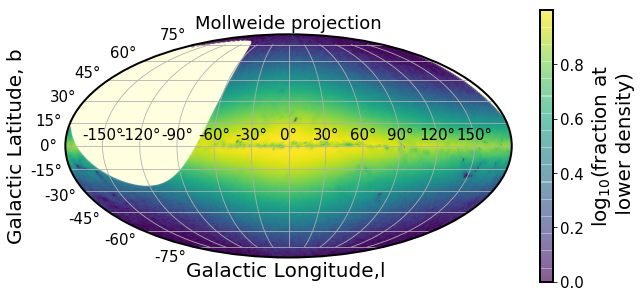
\includegraphics[width=1.0\columnwidth]{figs/01_MAF_densities.png}
%\vskip -0.15in
\caption{Galfast healpixels plotted in galactic coordinates in Mollweide projection. The brightest regions correspond to highest stellar densities. The missing part in the higher declination is the part of the sky above $\delta>40 \degree$, which is not observable from the southern location of Cerro Pach\'on.}
\label{fig:MAF_densities}
\end{figure} 
%### add exclusion / confusion zone on top of the MAF Galfast count?   

To match the LSST single-visit depth,  we select magnitude bins smaller than r=24.5.   For each healpixel we calculate the number of pixels that have a higher stellar count.  Since each healpixel has an equal area, the fraction of pixel number above a certain threshold corresponds to the fraction of sky area above given density limit.  Fig.~\ref{fig:illustrate_density} illustrates how we define percentiles of stellar densities, so that eg. 'top 1\%' density means that only 1 in 100 pixels has a higher density than a given pixel, and 'top 10\%' means that '10 \%' of pixels in the considered simulation of the sky. 

\begin{figure}
\centering
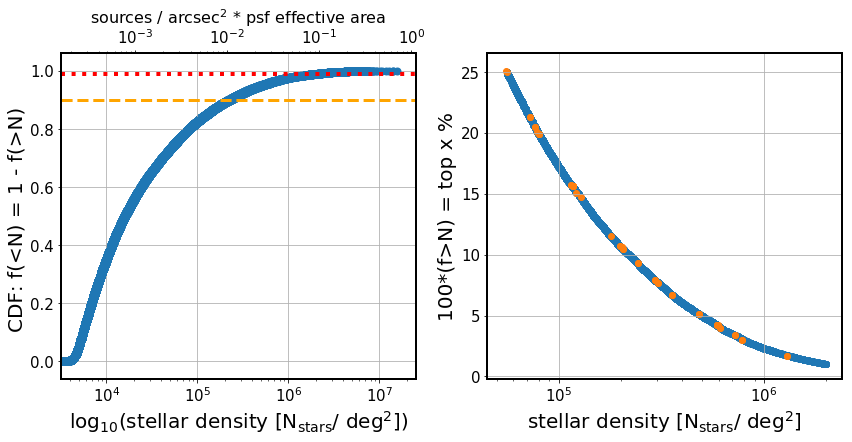
\includegraphics[width=0.95\columnwidth]{figs/MAF_density_definitions.png}
%\vskip -0.15in
\caption{Using the Galfast sky simulation to choose DECAPS fields sampliong different density regions.  The left panel shows  the stellar density as a function of the fraction of the sky at smaller density.  It is equivalent to the cumulative distribution function. Given the stellar density per simulated healpixel, we count the number of healpixels at greater density. Normalized to the number of pixels, given their equal area, it corresponds to the fraction of the sky at greater stellar density. Horizontal dashed lines illustrate selecting pixels at top 1\% or 10\% density. 
The right panel focuses on the 1-CDF, converted to \% , between 1 and 25\%.  
It implies that according to the simulation , the density of 200 000 stars per sq.deg. corresponds to 5\% of the sky, and only  1\% of the sky has more than $10^{6}$ stars per sq.deg. 
The upper axis represents the dimensionless demnsity parameter $N_{beam} = N_{stars}/{arcsec}^{2} * A_{PSF}$, with the PSF effective area $A_{PSF} = 0.64 {arcsec}$.}
\label{fig:illustrate_density}
\end{figure} 




We illustrate the location of pixels representative of various density brackets on the sky in Fig.~\ref{fig:mollw_galactic}. 


\begin{figure}
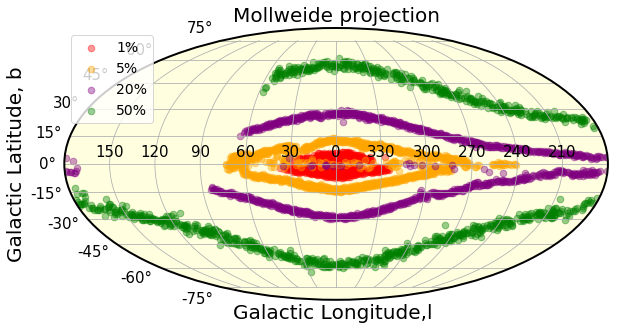
\includegraphics[width=1.0\columnwidth]{figs/03_density_regions_mollw_galactic.png}
%\vskip -0.15in
\caption{Illustration of location of regions representative of different relative simulated stellar densities in cylindrical projection, galactic coordinates. The x\% region  here means  x $\pm$ 1\%, eg.  5\% includes regions between 4-6\%. The highest density regions are located close to the galactic bulge, and regions of approximately constant stellar density trace isophotes of the Milky Way. The 20\% regions close to the galactic equator correspond to high extinction regions that appear to have less counts due to interstellar dust. The galactic exclusion zone in LSST is closely follows the 5\% region outline. }
\label{fig:mollw_galactic}
\end{figure} 


\section{DECam Plane Survey }
\label{sec:DECAPS}
To analyze the performance of the LSST Stack with real data, we used the Dark Energy Camera (DECam) imaging, taken as part of the  DECam Plane Survey (DECAPS)~\cite{schlafly2017}, at the 4-m Cerro Tololo Inter-American Observatory telescope (CTIO)\footnote{see \url{http://www.ctio.noao.edu/noao/node/1033}}. On Fig.~\ref{fig:decaps_fields} we overlay the locations of all DECAPS fields on top  the MAF map of the LSST sky. All DECAPS single-epoch images were processed with the DECAPS pipeline, resulting in single-epoch catalogs. The details of DECAPS pipeline can be found in Schlafly et al. 2017~\cite{schlafly2017}. DECAPS pipeline was specifically designed for crowded field photometry. It performs DAOPhot-like procedure ~\ref{stetson1987}, but does not use DAOPhot. The algorithm performs repeated source detection, subtraction, and re-detection, which is different from the LSST pipeline. DECAPS pipeline simultaneously solves for the positions and fluxes for all stars for a small fragment of the CCD (see Sec.4 in ~\cite{schlafly2017}).  The headers of all DECAPS catalogs were assembled into the image database that contains information about single-visit exposure time, filter,  time of observation, position, etc. We used the image database to select DECAPS fields with single-epoch depth similar to that of the single-visit depth of 30 sec LSST  r-band exposure. Thus we selected DECAPS fields with  exposure between 90  and 125 sec, taken in   u, g, r,  or VR filter. 

\begin{figure}
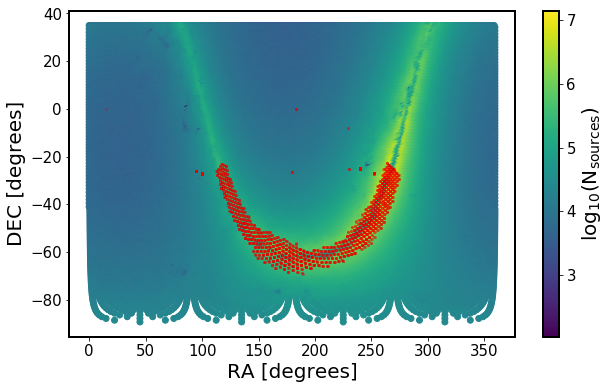
\includegraphics[width=1.0\columnwidth]{figs/04_MAF_DECAPS_sources.png}
%\vskip -0.15in
\caption{All DECAPS fields, overlaid on the map of healpixel stellar densities from MAF simulated sky.  We matched the position of the center of each DECAPS field to the nearest healpixel to obtain an estimate of stellar density at each DECAPS field. In this way we selected DECAPS fields representative of various stellar densities (eg. 5\%, 10\%, 15\%, as explained in Sec.~\ref{sec:MAF}). }
\label{fig:decaps_fields}
\end{figure} 


We cross-matched the DECAPS image database with the  stellar density information contained in MAF healpixels. Each DECAPS image plane is tiled by a mosaic of 62 CCDs\footnote{See Fig.4-3 in the NOAO Data Handbook ~\citep{shaw2015}}. The size of each CCD element of the DECAm image plane mosaic is 2046x4094 pixels, with pixel scale of 0.27 arcsec / px , so that a single mosaic element covers an area of 0.047117 square \degree. A single DECam exposure is also called a visit, and with 62 mosaic elements the full field of view  2.2\degree wide is several times bigger than the full moon. This makes it comparable to the LSST 3.5\degree wide field of view.  Using the coordinates of the center of each DECAPS field  we found the nearest healpixel within 0.5\degree . 


\begin{figure}
\centering
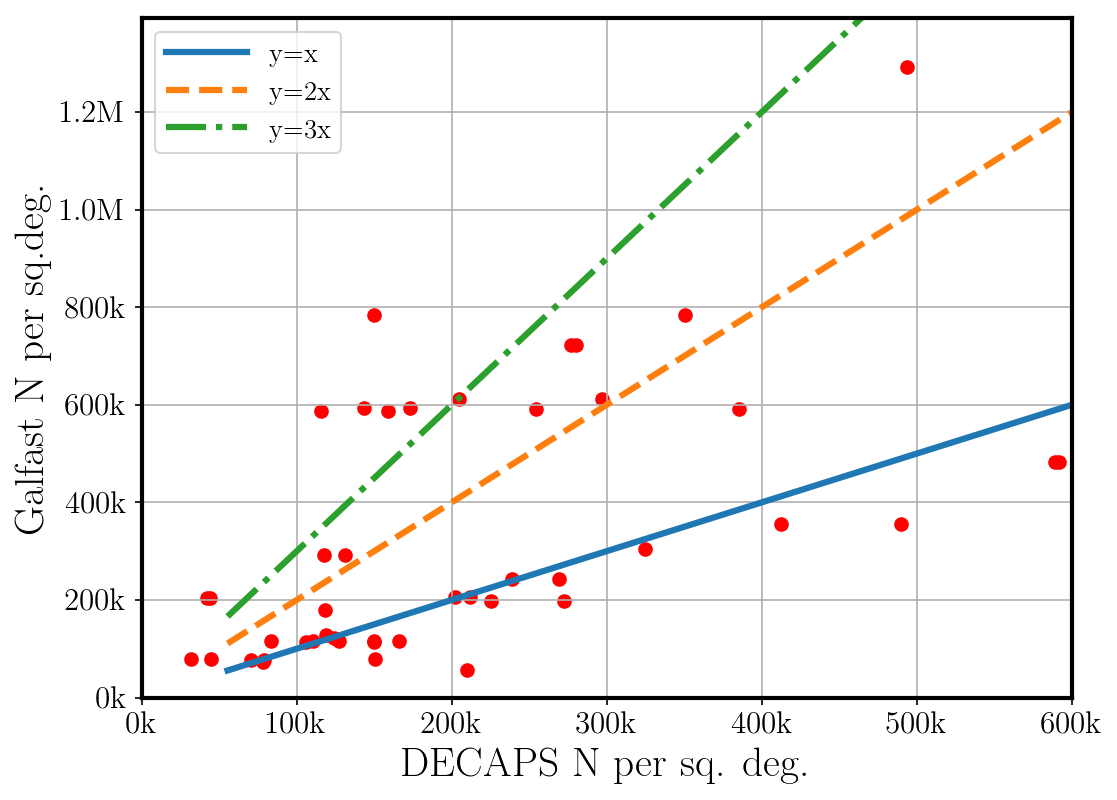
\includegraphics[width=0.75\columnwidth]{figs/MAF_DECAPS_comparison.png}
%\vskip -0.15in
\caption{Comparison of DECAPS counts to Galfast simulated stellar counts.  Overplotted are the line of equivalence y=x, and its multipicities (2x,3x). It shows that the simulation may be not more accurate than up to a factor of a few, but it is nevertheless useful for defining density regions. Part of the reason for discrepancy could be the order-of-magnitude nature of the experiment - Galfast counts here assume the single-visit depth of 24.5 mag in r-band. The DECAPS exposure time ($\approx$100 sec) and filter (g, or r) were chosen to mimic that depth as closely as possible, but the regions targeted include much extinction, which means that in some cases DECAPS counts may be less than what is  implied by the simulation. Different zero-point magnitude dependent on seeing conditions could also contribute to the depth probed by DECAPS.  However, there is a number of fields that lie along the blue line, implying that in some cases the Galfast counts were very close to the true counts.}
\label{fig:maf_decaps_compare}
\end{figure} 

\begin{figure}
\begin{centering}
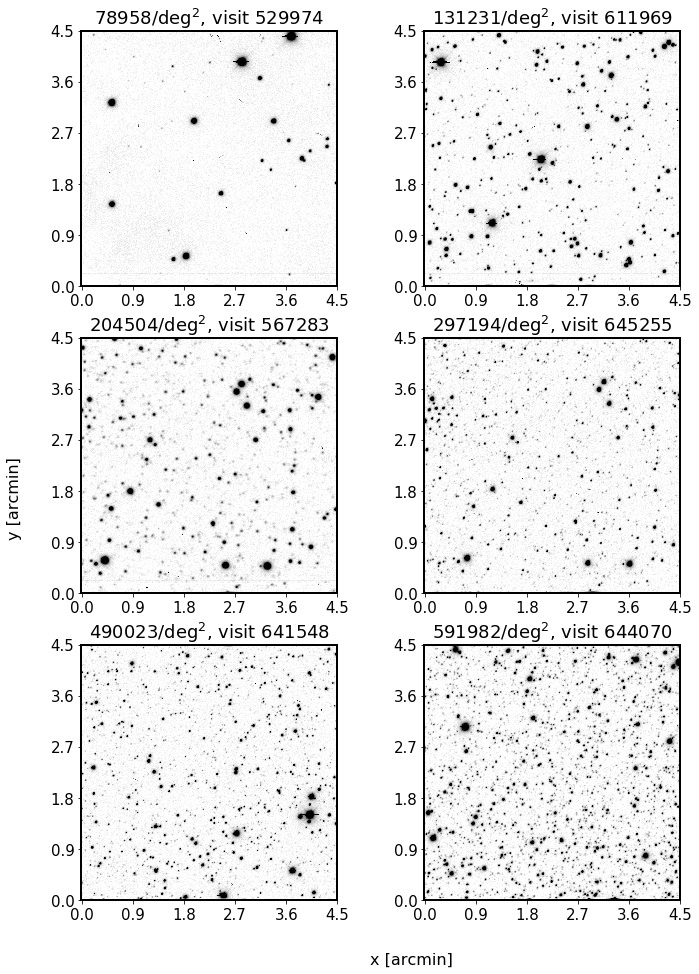
\includegraphics[width=0.85\columnwidth]{figs/Illustrate_densities_DECAPS.png}
%\vskip -0.15in
\caption{Illustration of regions of different stellar count in the cleaned DECAPS single-epoch catalogs. As shown on Fig.~\ref{fig:maf_decaps_compare}, the Galfast count (and therefore \% level), does not always correspond 1:1 to the actual reported DECAPS stellar count. For this reason we simply ordered all DECAPS fields in terms of source count, and display postage stamp miniatures of CCD regions for visits in regions of increasing stellar density. }
\label{fig:decaps_illustrate_densities}
\end{centering}
\end{figure} 


\section{LSST Processing of DECAPS data}
\label{sec:LSST}
The calibrated DECAPS imaging was processed with the LSST Science Pipelines installed on the LSST-dev machine at the NCSA\footnote{\url{lsst-dev01.ncsa.illinois.edu} (141.142.237.49) OS: CentOS 7.4.1708   HW: Dell Inc. CPU: 48x 2.60GHz RAM: 252 GB}, with Stack version d\_2017\_10\_27\footnote{\url{https://eups.lsst.codes/stack/src/tags/}}.  We specifically employed processCcd.py and the standard Stack configuration. Transferring the resulting source catalogs and calexp files to a local machine we analyzed the output of LSST processing using jupyter notebooks and custom python tools. 

To compare single epoch DECAPS catalogs to LSST source catalogs we used the image mask, deblender flags, and other quality flags. The cleaning process is described in this section. 

%The big picture is to find how metrics that we develop behave as a function of source crowdedness. We consider completeness, and photometric accuracy. 

\subsection{Cleaning DECAPS catalog, comparison to LSST pixel mask}
\label{sec:clean_decaps}
To compare LSST and DECAPS catalogs, we cleaned both catalogs using the flag information assigned to each source by the respective image processing pipeline. To verify the validity of DECAPS source flags, we compared them with the LSST pixel-level mask information stored in the FITS Header Data Unit. Pixel-level masks are encoded in 8 bits,  each of which can be 'on' or 'off', signifying that a given flag was 'on' or 'off' for a given pixel. The total value of the mask at each pixel is a decimal representation of such eight bits binary number, eg.  $(00100001)_{2} = 2^{0} + 2^{5}  = 1 + 32 = (33)_{10} $ means that bit $'0'$ and $'5'$ are 'on' (counting from the right). See Table~\ref{tab:lsst_flags} for details. 


\begin{table}
\centering
\caption{LSST pixel mask bit values.}
\label{tab:lsst_flags}
\begin{tabular}{ ccc} 
\hline
Bit position & Description & Mask decimal value  \\ 
\hline
0  & bad               & 1    \\ 
1  & saturated         & 2   \\ 
2  & interpolated      & 4    \\ 
3  & cosmic ray        & 8    \\ 
4  & edge              & 16    \\ 
5  & detected          & 32   \\ 
6  & detected negative & 64   \\ 
7  & suspect           & 128   \\ 
8  & no data           & 256     \\ 
\hline
\end{tabular}
\end{table}

For each  visit we considered DECAPS single-epoch source catalog, and the LSST calexp image. We combined the calexp image mask value at the nearest pixel to every DECAPS source given its pixel coordinates.  The bitwise 'and' of image mask with mask filter $(11011111)_{2} = (2^{1}+2^{2}+2^{3}+2^{4}+2^{6}+2^{7})_{10}$ (see Table~\ref{tab:lsst_flags} for details ), flagged the source   as 'bad' if either of the flag bits apart from '5' (detected) was 'on'. 

\begin{table}
\centering
\caption{DECAPS flags. We excluded sources with flag bits 1,3,4,5,6,8,20,22.}
\label{tab:decaps_flags}
\begin{tabular}{ ccc} 
\hline
Bit position & Description \\ 
\hline
1  &     Bad pixel            \\ 
3  &    Saturated      \\ 
4  &    Bleed trail      \\ 
5  &    Cosmic ray       \\ 
6  &    Low weight      \\ 
8  &    Long streak      \\ 
20  &   Additional bad pixel    \\ 
21 &    Nebulosity     \\ 
22  &   S7 amplifier B        \\ 
\hline
\end{tabular}
\end{table}

Apart from LSST flags, each source also has a DECAPS pipeline flag, the value of which is made up of of bits inherited from the NOAO Community Pipeline (see Table~\ref{tab:decaps_flags}). We performed a bitwise 'and' of DECAPS flags with the mask filter $(2^{1}+ 2^{3}+  2^{4}+  2^{5}+  2^{6}+  2^{8}+  2^{20}+  2^{22})_{10}$, flagging the source as 'bad' if either of these mask bits were 'on'. 

Given the LSST and DECAPS flags, we compared which sources would be excluded based on the DECAPS source-level flags vs LSST pixel-level masks. We found for a random visit  611980  that the overlap between sources excluded by LSST pixel mask information versus DECAPS source flags is 99\%.  This means that the DECAPS flagging is consistent with the LSST image mask information, and the same sources would be 'excluded' based on either DECAPS flags or LSST mask information. For this reason we decided to clean the DECAPS catalog with  source level flags, rather than the LSST image mask data. 
 
\subsection{Cleaning the LSST catalog}
\label{sec:clean_lsst}
The LSST source catalog contains for each source a list of flags that could be set 'on' or 'off'. Of these, flags labeled \verb|base_PixelFlags_flag| contain information relevant to the level of source detection, rather than processing (see Table~\ref{tab:lsst_src_flags}).

\begin{table}
\centering
\caption{LSST source flags explanation.}
\label{tab:lsst_src_flags}
\begin{tabular}{cl}
\hline
name & explanation \\
\hline
flag & general failure flag, set if anything went wrong \\
offimage & Source center is off image \\
edge & Source is outside usable exposure region  \\
interpolated & Interpolated pixel in the Source footprint \\
saturated & Saturated pixel in the Source footprint \\
cr & Cosmic ray in the Source footprint \\
bad & Bad pixel in the Source footprint \\
suspect & Source's footprint includes suspect pixels \\
interpolatedCenter & Interpolated pixel in the Source center \\
saturatedCenter & Saturated pixel in the Source center \\
crCenter & Cosmic ray in the Source center \\
suspectCenter & Source's center is close to suspect pixels \\
flag & General Failure Flag \\
\hline
\end{tabular}
\end{table}

We clean the LSST source catalog by removing sources that have flags 'edge' or 'interpolatedCenter'\footnote{This is similar to the example in Sec.4 of SDSS Image Processing I: The Deblender~\citep{lupton2005}}. Other flags would remove too many sources that have only small defects, eg. flag 'interpolated' may be on for a bright source across the footprint of which there is a cosmic ray, while flag 'bad' may be on for any source which has even one bad pixel in the footprint. A comparison of the initial source count to the final source count (after cleaning) is shown on Fig.~\ref{fig:lsst_count_comparison}, with detailed counts in  Table ~\ref{tab:lsst_summary}.


\begin{landscape}
\begin{longtable}{cccccccccccc}
Visit & $N_{raw}$ & $(N_{f})$ & $-N_{r}$ & $=N_{c}$ & $N_{c}$/deg$^{2}$ & $N_{MAF}$/deg$^{2}$ & $\rho_{MAF}$ & $N_{loSN}$ & $N_{parents}$ & $N_{blended}$ & $N_{deblended}$ \\
568172 & 29809 & 9148 & 12434 & 17375 & 6241 & 72072 & 21.3 & 12986 & 153919 & 77723 & 289200 \\
527319 & 120862 & 13744 & 39638 & 81224 & 29175 & 79632 & 19.9 & 34282 & 112848 & 28212 & 86196 \\
530012 & 160406 & 15210 & 61337 & 99069 & 35585 & 203040 & 10.6 & 51669 & 20425 & 2143 & 7241 \\
525846 & 167582 & 15247 & 63295 & 104287 & 37459 & 203040 & 10.6 & 51949 & 96932 & 31724 & 113865 \\
525900 & 171337 & 15037 & 58219 & 113118 & 40631 & 79632 & 19.9 & 46796 & 70011 & 9731 & 41120 \\
529989 & 182933 & 15910 & 61808 & 121125 & 43508 & 79632 & 19.9 & 49120 & 114760 & 54746 & 198511 \\
529974 & 228849 & 16842 & 67339 & 161510 & 58014 & 76572 & 20.5 & 44712 & 104406 & 26981 & 103920 \\
525814 & 235307 & 16811 & 72214 & 163093 & 58582 & 76572 & 20.5 & 50998 & 98063 & 28128 & 102658 \\
527096 & 227256 & 16100 & 59686 & 167570 & 60191 & 55908 & 25.0 & 36748 & 85483 & 16136 & 69718 \\
644125 & 242521 & 16387 & 72363 & 170158 & 60101 & 72072 & 21.3 & 40731 & 89237 & 17861 & 75835 \\
611980 & 273032 & 18816 & 76043 & 196989 & 70758 & 116856 & 15.6 & 41383 & 78662 & 42516 & 151854 \\
527247 & 264383 & 15283 & 66539 & 197844 & 71065 & 116676 & 15.6 & 38391 & 138758 & 59728 & 200438 \\
567283 & 280305 & 16981 & 68379 & 211926 & 76123 & 612648 & 4.0 & 30908 & 230049 & 64593 & 195501 \\
527555 & 313294 & 1173 & 81585 & 231709 & 83229 & 783324 & 3.0 & 39458 & 127709 & 49579 & 170745 \\
612757 & 317270 & 4014 & 84877 & 232393 & 82084 & 292788 & 7.9 & 42468 & 128543 & 50645 & 176673 \\
527246 & 319929 & 18136 & 86268 & 233661 & 83930 & 114588 & 15.7 & 47233 & 128325 & 58651 & 206903 \\
640891 & 355861 & 24520 & 107462 & 248399 & 87737 & 121536 & 15.1 & 60163 & 127665 & 45693 & 146571 \\
611970 & 377917 & 26716 & 120640 & 257277 & 92413 & 178992 & 11.5 & 80884 & 133384 & 53522 & 184423 \\
645251 & 348033 & 18786 & 89669 & 258364 & 91257 & 128016 & 14.7 & 41210 & 129397 & 34130 & 100856 \\
527296 & 361951 & 21167 & 101452 & 260499 & 93571 & 588096 & 4.2 & 63149 & 144777 & 50631 & 182509 \\
611969 & 387056 & 25752 & 118639 & 268417 & 96415 & 292788 & 7.9 & 74291 & 162439 & 70305 & 262885 \\
526413 & 368017 & 22267 & 98745 & 269272 & 96722 & 78480 & 20.1 & 52626 & 151602 & 82678 & 295547 \\
525838 & 371329 & 19984 & 100644 & 270685 & 97229 & 116676 & 15.6 & 54839 & 71782 & 16117 & 79683 \\
525837 & 393879 & 22350 & 107414 & 286465 & 102898 & 114588 & 15.7 & 56743 & 74171 & 14580 & 71655 \\
611529 & 398924 & 22625 & 105677 & 293247 & 105334 & 116856 & 15.6 & 54741 & 113152 & 86539 & 376291 \\
527552 & 395446 & 1716 & 99214 & 296232 & 106406 & 591336 & 4.2 & 44093 & 95415 & 72727 & 318061 \\
525920 & 415231 & 22439 & 111423 & 303808 & 109127 & 588096 & 4.2 & 59375 & 133660 & 55280 & 198116 \\
527300 & 436689 & 24839 & 120330 & 316359 & 113635 & 594324 & 4.2 & 70470 & 170980 & 82687 & 317507 \\
644035 & 435830 & 2170 & 106363 & 329467 & 116371 & 205308 & 10.5 & 46535 & 93985 & 48307 & 174978 \\
525904 & 479294 & 26679 & 135534 & 343760 & 123478 & 594324 & 4.2 & 77080 & 112960 & 67743 & 255127 \\
527453 & 495629 & 28732 & 139172 & 356457 & 128039 & 242316 & 9.3 & 80487 & 208259 & 137811 & 565651 \\
609754 & 490143 & 26233 & 121738 & 368405 & 132330 & 116856 & 15.6 & 62319 & 199832 & 151565 & 653749 \\
530032 & 486203 & 23112 & 115217 & 370986 & 133257 & 198432 & 10.7 & 51002 & 176645 & 113085 & 441312 \\
526152 & 520842 & 28739 & 143336 & 377506 & 135599 & 55404 & 25.1 & 77724 & 142876 & 100061 & 400366 \\
567795 & 508405 & 26663 & 129592 & 378813 & 136069 & 721728 & 3.4 & 63447 & 62120 & 42489 & 175696 \\
641497 & 529827 & 28546 & 137626 & 392201 & 138530 & 205308 & 10.5 & 59868 & 184493 & 139641 & 592661 \\
640995 & 571174 & 2973 & 155705 & 415469 & 146748 & 242316 & 9.3 & 85262 & 171899 & 67666 & 239729 \\
527064 & 558264 & 26197 & 132299 & 425965 & 153006 & 591336 & 4.2 & 56098 & 184352 & 59068 & 193269 \\
566793 & 560376 & 1088 & 134186 & 426190 & 158458 & 1292976 & 1.7 & 59842 & 132416 & 60622 & 222193 \\
644205 & 571378 & 4663 & 142463 & 428915 & 151498 & 721728 & 3.4 & 65955 & 165636 & 45858 & 150457 \\
525879 & 575982 & 28502 & 139102 & 436880 & 156927 & 198432 & 10.7 & 63181 & 119515 & 85247 & 353502 \\
644144 & 597726 & 30439 & 152632 & 445094 & 168442 & 1292976 & 1.7 & 77506 & 115951 & 62116 & 217379 \\
644082 & 614401 & 29828 & 152226 & 462175 & 163246 & 783324 & 3.0 & 65428 & 166750 & 94046 & 356549 \\
645255 & 617345 & 2342 & 148062 & 469283 & 165756 & 612648 & 4.0 & 62971 & 187074 & 140722 & 589579 \\
644011 & 643303 & 5962 & 151827 & 491476 & 173595 & 355896 & 6.7 & 58686 & 129561 & 76106 & 302738 \\
641500 & 731042 & 2925 & 178763 & 552279 & 195071 & 305280 & 7.7 & 78451 & 171114 & 92824 & 350463 \\
526028 & 911721 & 38810 & 234490 & 677231 & 243260 & 305280 & 7.7 & 113255 & 166673 & 85331 & 319374 \\
644074 & 916795 & 41973 & 219530 & 697265 & 246282 & 481788 & 5.1 & 89471 & 102816 & 48459 & 162019 \\
644070 & 917375 & 3993 & 214363 & 703012 & 248312 & 481788 & 5.1 & 87108 & 122274 & 89793 & 385659 \\
641548 & 1005146 & 44347 & 238787 & 766359 & 270687 & 355896 & 6.7 & 96812 & 117637 & 85174 & 357565 \\

\hline

\caption{A summary of all LSST-processed DECAPS visits. The column `visit` corresponds to the DECAPS visit number.  The following four columns (`N raw`,  `N f`, `-N r`,  `=N c`) contain the source counts  per visit area ($\approx$ 2.74 deg$^{2}$). `N raw` is the input number of sources per visit , summing over all CCD source catalogs. `(N f)` is the number of sources removed due to bad flags. `-N r` is the total number of removed sources ( due to flags, low S/N, or sources that in the LSST deblending process are neither isolated parents, nor deblended children). `=N c` is the final number of clean sources per  visit (`N raw` - `N r`= `N c`). `N c/deg$^{2}$` is `=N c` converted to count per deg$^{2}$. N MAF/deg$^{2}$ is the predicted number of sources per deg$^{2}$ at that location based on Galfast simulation. $\rho_{MAF}$ is the  MAF density; eg. 21.3 is the top 21.3\% stellar density of the simulated sky.}
\label{tab:lsst_summary}
\end{longtable}
\end{landscape}
%\end{tabular}
%\end{table}


%\begin{table}
%\centering
\begin{longtable}{cccccccc}
%\begin{tabular}
Visit & $N_{raw}$ & $(N_{f})$ & $-N_{r}$ & $=N_{c}$ & $N_{c}$/deg$^{2}$ & $N_{MAF}$/deg$^{2}$ & $\rho_{MAF}$ \\
568172 & 16824 & 138 & 150 & 16674 & 5989 & 72072 & 21.3 \\
527319 & 92326 & 2819 & 3039 & 89287 & 32071 & 79632 & 19.9 \\
530012 & 121313 & 3293 & 3982 & 117331 & 42145 & 203040 & 10.6 \\
525846 & 125245 & 3135 & 3457 & 121788 & 43746 & 203040 & 10.6 \\
525900 & 127722 & 2557 & 2786 & 124936 & 44876 & 79632 & 19.9 \\
529989 & 140043 & 2527 & 2803 & 137240 & 49296 & 79632 & 19.9 \\
527096 & 194837 & 2126 & 2290 & 192547 & 69162 & 55908 & 25.0 \\
525814 & 200562 & 4481 & 4938 & 195624 & 70268 & 76572 & 20.5 \\
529974 & 224231 & 3992 & 4413 & 219818 & 78958 & 76572 & 20.5 \\
644125 & 228088 & 5570 & 6182 & 221906 & 78380 & 72072 & 21.3 \\
527247 & 237656 & 4858 & 5144 & 232512 & 83518 & 116676 & 15.6 \\
527246 & 301083 & 5469 & 5907 & 295176 & 106027 & 114588 & 15.7 \\
611980 & 315722 & 6779 & 7397 & 308325 & 110750 & 116856 & 15.6 \\
527296 & 330295 & 7176 & 7726 & 322569 & 115866 & 588096 & 4.2 \\
611970 & 340528 & 9668 & 10513 & 330015 & 118541 & 178992 & 11.5 \\
612757 & 342629 & 8541 & 9473 & 333156 & 117674 & 292788 & 7.9 \\
645251 & 343358 & 5546 & 6253 & 337105 & 119069 & 128016 & 14.7 \\
640891 & 361837 & 9423 & 10389 & 351448 & 124135 & 121536 & 15.1 \\
525838 & 360793 & 6057 & 6515 & 354278 & 127256 & 116676 & 15.6 \\
611969 & 376588 & 10280 & 11243 & 365345 & 131231 & 292788 & 7.9 \\
527300 & 409385 & 8974 & 9654 & 399731 & 143583 & 594324 & 4.2 \\
611529 & 428299 & 9981 & 11167 & 417132 & 149833 & 116856 & 15.6 \\
527555 & 421706 & 3848 & 4285 & 417421 & 149937 & 783324 & 3.0 \\
525837 & 425261 & 6791 & 7437 & 417824 & 150082 & 114588 & 15.7 \\
526413 & 428035 & 8417 & 9137 & 418898 & 150467 & 78480 & 20.1 \\
525920 & 449868 & 6675 & 7430 & 442438 & 158923 & 588096 & 4.2 \\
609754 & 474355 & 10034 & 11677 & 462678 & 166193 & 116856 & 15.6 \\
525904 & 490306 & 8413 & 9118 & 481188 & 172842 & 594324 & 4.2 \\
567283 & 575760 & 5549 & 6426 & 569334 & 204504 & 612648 & 4.0 \\
644035 & 583432 & 9457 & 10948 & 572484 & 202208 & 205308 & 10.5 \\
526152 & 599164 & 12579 & 14023 & 585141 & 210182 & 55404 & 25.1 \\
641497 & 611424 & 10156 & 11324 & 600100 & 211962 & 205308 & 10.5 \\
530032 & 638179 & 9776 & 10964 & 627215 & 225295 & 198432 & 10.7 \\
527453 & 682113 & 14654 & 16569 & 665544 & 239062 & 242316 & 9.3 \\
527552 & 714305 & 6031 & 6893 & 707412 & 254101 & 591336 & 4.2 \\
525879 & 772457 & 11625 & 13117 & 759340 & 272754 & 198432 & 10.7 \\
640995 & 783011 & 17946 & 20850 & 762161 & 269204 & 242316 & 9.3 \\
567795 & 791019 & 9439 & 11056 & 779963 & 280162 & 721728 & 3.4 \\
644205 & 800175 & 13601 & 15899 & 784276 & 277016 & 721728 & 3.4 \\
645255 & 852539 & 9620 & 11135 & 841404 & 297194 & 612648 & 4.0 \\
641500 & 935661 & 14131 & 16133 & 919528 & 324788 & 305280 & 7.7 \\
644082 & 1007998 & 12826 & 15633 & 992365 & 350515 & 783324 & 3.0 \\
526028 & 1035808 & 17929 & 20772 & 1015036 & 364600 & 305280 & 7.7 \\
527064 & 1085375 & 10200 & 12399 & 1072976 & 385412 & 591336 & 4.2 \\
644011 & 1181972 & 11059 & 13806 & 1168166 & 412611 & 355896 & 6.7 \\
566793 & 1350724 & 12414 & 22431 & 1328293 & 493863 & 1292976 & 1.7 \\
641548 & 1404895 & 14336 & 17562 & 1387333 & 490023 & 355896 & 6.7 \\
644144 & 1444897 & 16255 & 28641 & 1416256 & 535971 & 1292976 & 1.7 \\
644074 & 1692430 & 16941 & 23670 & 1668760 & 589427 & 481788 & 5.1 \\
644070 & 1698554 & 16404 & 22559 & 1675995 & 591982 & 481788 & 5.1 \\
\hline
\caption{A summary of all single-epoch DECAPS source catalogs, with columns as in  Table ~\ref{tab:lsst_summary}. See Fig.~\ref{fig:lsst_count_comparison} comparing the 'N raw' converted to number of sources per square degree, and  'N clean per sq.deg.'.  }
\label{tab:decaps_summary}
\end{longtable}
%\end{tabular}
%\end{table}


\begin{figure}
\begin{centering}
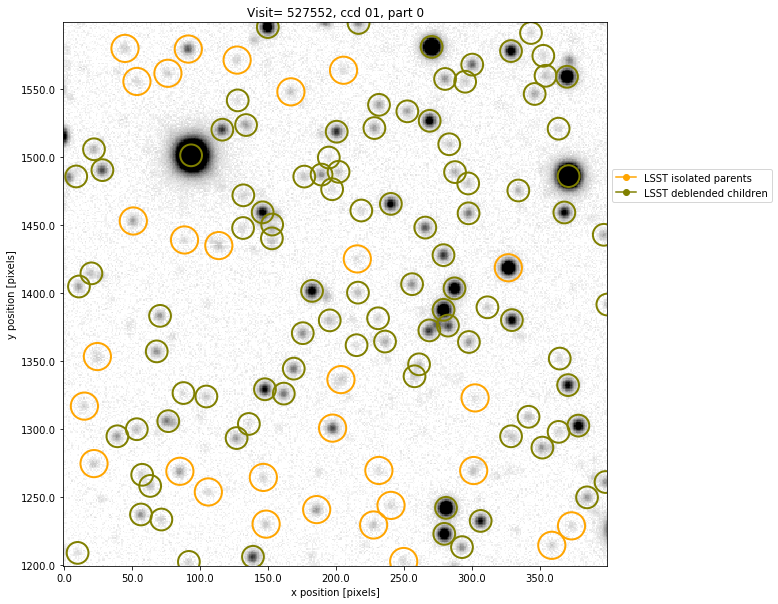
\includegraphics[width=1.0\columnwidth]{figs/visit_527552_ccd_1.png}
\caption{We illustrate the sources as reported by the LSST pipeline for a small region of CCD01 of visit 527552. A source may be reported as an isolated source (yellow),  or a successfully deblended child (green). In this analysis we only keep isolated parents or deblended children.}
\label{fig:lsst_sources}
\end{centering}
\end{figure} 


\begin{figure}
\begin{centering}
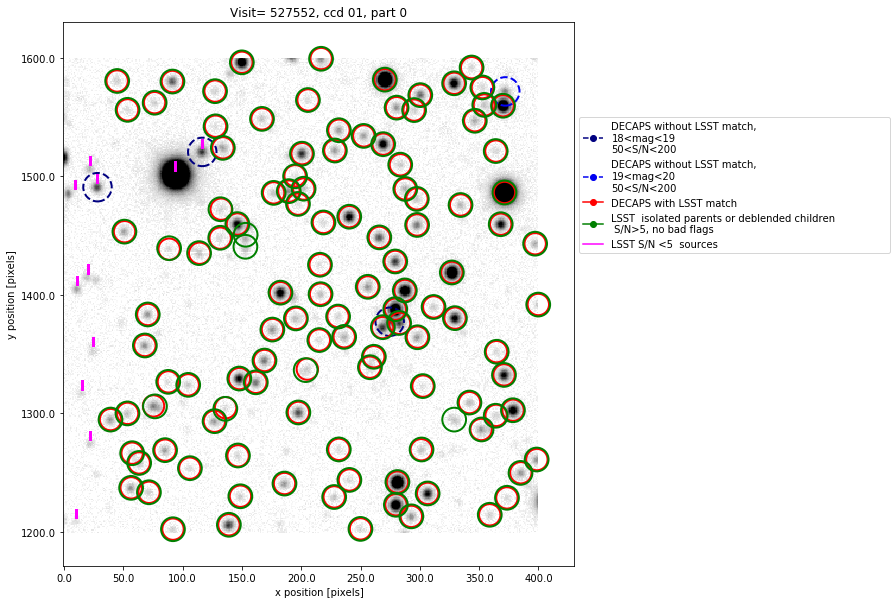
\includegraphics[width=1.0\columnwidth]{figs/visit_527552_ccd_1_lowSN.png}
\caption{The same region as on Fig.~\ref{fig:lsst_sources}. Green circles mark the position of retained LSST sources: isolated parents, or deblended children, with  S/N > 5, and no bad flags. Red circles mark the position of DECAPS detections with an LSST match. Vertical magenta dashes are above the LSST sources with S/N < 5.   Blue dashed circles mark location of DECAPS source without an LSST match. Note that eg. at (x,y) = 50,1490  an LSST source was detected, but since its  S/N < 5 it was not kept in the clean LSST catalog.   }
\label{fig:lsst_decaps_sources}
\end{centering}
\end{figure} 


\begin{figure}
\begin{centering}
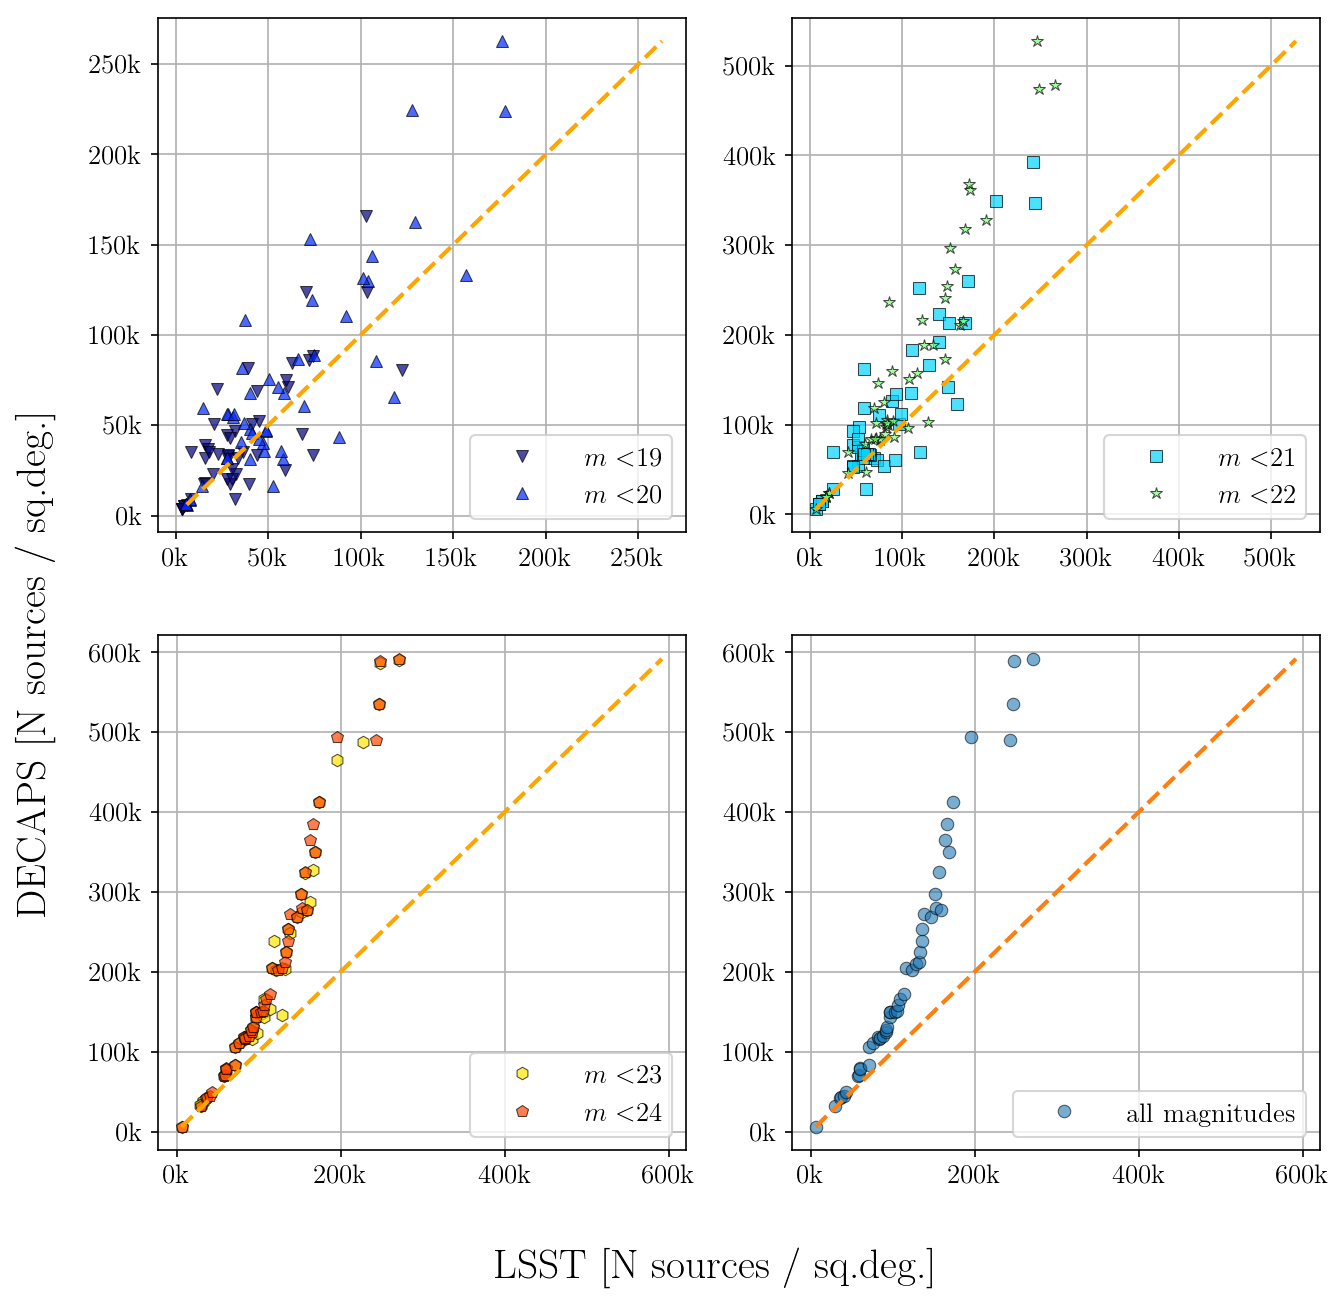
\includegraphics[width=0.9\columnwidth]{figs/decaps_lsst_source_count.png}
%\vskip -0.15in
\caption{A plot of source count comparing LSST to DECAPS source catalogs of the same fields (visits). 
On each panel we plot the number of counts up to a given magnitude, increasing the depth clockwise. 
The bottom right panel shows all sources without magnitude limits. For exact counts in each stellar field, see  Tables ~\ref{tab:lsst_summary} and Table ~\ref{tab:decaps_summary}.}
\label{fig:lsst_count_comparison}
\end{centering}
\end{figure} 


Given the single-epoch DECAPS source catalogs, and the LSST source catalogs, we followed a uniform set of procedures to clean both datasets, and in turn cross-match positionally. First we made a quality cut removing all sources with signal-to-noise ratio smaller than five:  $S/N < 5$. The number of sources thus removed depends on a visit number, but does not exceed few \% of the catalog. Following that we also removed sources with flags that correspond to bad, edge detections, cosmic rays, or saturation spikes (as outlined in Sec.~\ref{sec:clean_decaps} and ~\ref{sec:clean_lsst}). The LSST Processing Pipeline deblends sources in a similar fashion to the SDSS Imaging Pipeline\footnote{SDSS Image Processing I: The Deblender~\citep{lupton2005}, SDSS Image Processing II: The Photo Pipelines~\citep{lupton2001},~\citep{lupton2002}, and ~\citep{lupton2005a}}.   For the LSST source catalog,  we chose to keep only those sources that were either isolated parents ( parentId=0, nchild=0), or deblended children (parentId != 0 , nchild=0) (see Table ~\ref{tab:lsst_deblend} for details.)



\begin{table}
\centering
\caption{ Summary of possible parentId and nchild combinations for blended sources in the LSST Science Pipeline. An example count in the final column is provided for visit 525814, a top 20\% density region, which has the raw source count 235307. For that visit  16811 sources had bad flags, 49901  had S/N < 5, and in total 163093 were kept in the clean catalog.  }
\label{tab:lsst_deblend}
\begin{tabular}{cccccccc}
parentID & nchild & type  & decision &  count \\
0 & 0 & parent: isolated source & keep & 104406 \\
0 & >0 & blended source & remove & 26981 \\
!=0 & 0 & deblended child & keep  &103920\\
!=0 & >0 & failure case & remove & 0 \\
\hline
\end{tabular}
\end{table}


\section{Source detection and photometry}
\label{sec:metrics}

Starting with cleaned LSST and DECAPS source catalogs, we consider a set of metrics to compare the quality of LSST science pipelines to the  state-of-the-art DECAPS pipeline.  

\subsection{Completeness}

For each visit that corresponds to a given level of crowdedness, we consider the detection completeness of LSST to DECAPS. Assuming that DECAPS is the 'true' catalog of sources, we define completeness by the percentage of DECAPS sources (binned along DECAPS magnitude), that have an LSST match within 0.5 \arcsec. This is a very liberal requirement considering that for most visits >98\% of DECAPS sources have an LSST match within 0.3 \arcsec.  Second,  we require that the sources differ by not more than 0.5 magnitudes. As illustrated on Fig.~\ref{fig:dmag_scatter}, this only removes the outliers.  In fact, given that the majority of the sources (>99\%) that are matched within 0.5 \arcsec, do not differ by more than 0.5 magnitude, this constraint does not change the completeness by more than few \%.   Fig.~\ref{fig:completeness} shows how completeness , and catalog counts, depend on source density.


\begin{figure}
\begin{centering}
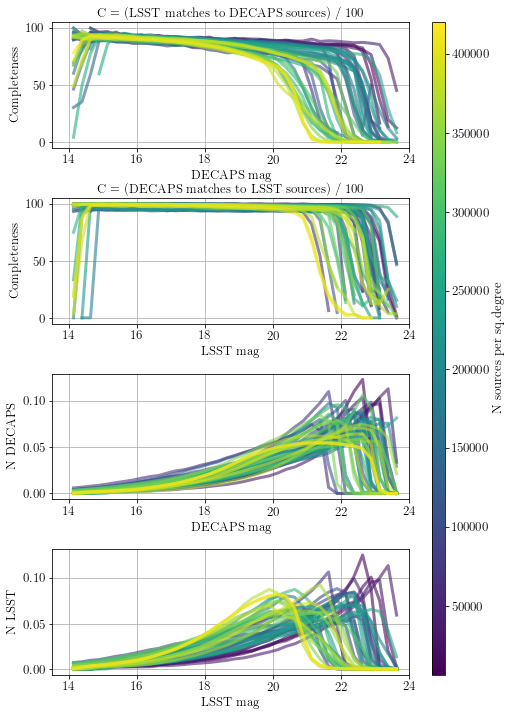
\includegraphics[width=0.75\columnwidth]{figs/completeness_4_panels_nomarker.png}
%\vskip -0.15in
\caption{Top two panels show source-to-source completeness.  The first panel is a measure of how complete is LSST catalog to DECAPS catalog (L-D),  i.e. the fraction of DECAPS sources per magnitude bin that have an LSST match.   The second panel shows an equivalent plot for the completeness of DECAPS to LSST (D-L), plotting the fraction of LSST sources that have a DECAPS match.  The bottom two panels show the normalized source counts  in the input catalogs. The LSST-DECAPS completeness falls off quicker than DECAPS-LSST, since DECAPS catalog has more sources at fainter magnitudes (see Fig.~\ref{fig:lsst_count_comparison}). Different colors correspond to different level of stellar crowdedness, expressed in terms of the number of sources per square degree in DECAPS clean catalogs.  We further characterize completeness by $\langle C_{18-20} \rangle$ - the mean completeness between 18-20 mag , and $m_{50}$ - the magnitude at which completeness falls to a 50\% level (see Fig.~\ref{fig:completeness_characterize}}
\label{fig:completeness}
\end{centering}
\end{figure} 


\begin{figure}
\begin{centering}
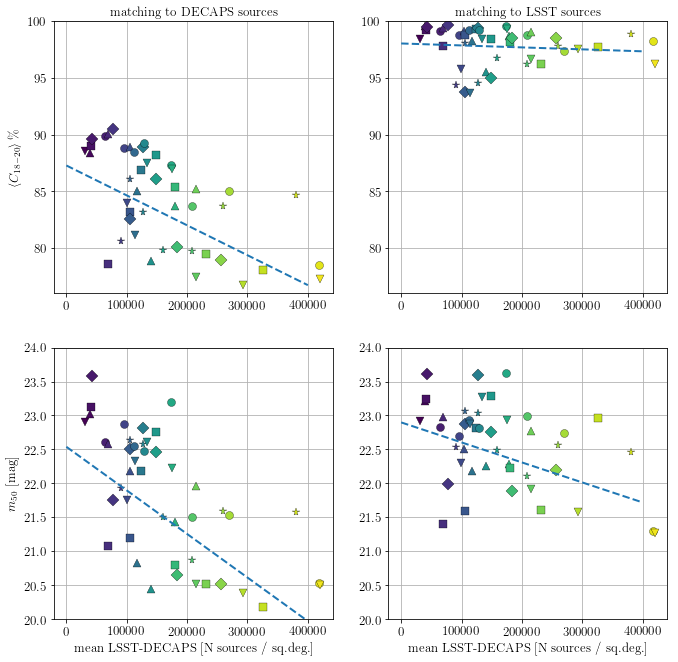
\includegraphics[width=0.96\columnwidth]{figs/decaps_lsst_c1820_m50.png}
%\vskip -0.15in
\caption{Magnitude at which completeness falls to 50\% (top two panels), and the mean completeness between 18 and 20 magnitudes (bottom two panels).  The panels on the left hand side correspond to the uppermost panel in Fig.~\ref{fig:completeness}, while the right hand side panels correspond to the second panel in Fig.~\ref{fig:completeness}. The color of all points corresponds to the stellar density, as in Fig.~\ref{fig:completeness}. In each panel we overplot the linear best-fit to indicate the expected overall trend of decreasing $\langle C_{18-20} \rangle$ and  $m_{50}$ with source density. }
\label{fig:completeness_characterize}
\end{centering}
\end{figure} 


\begin{figure}
\begin{centering}
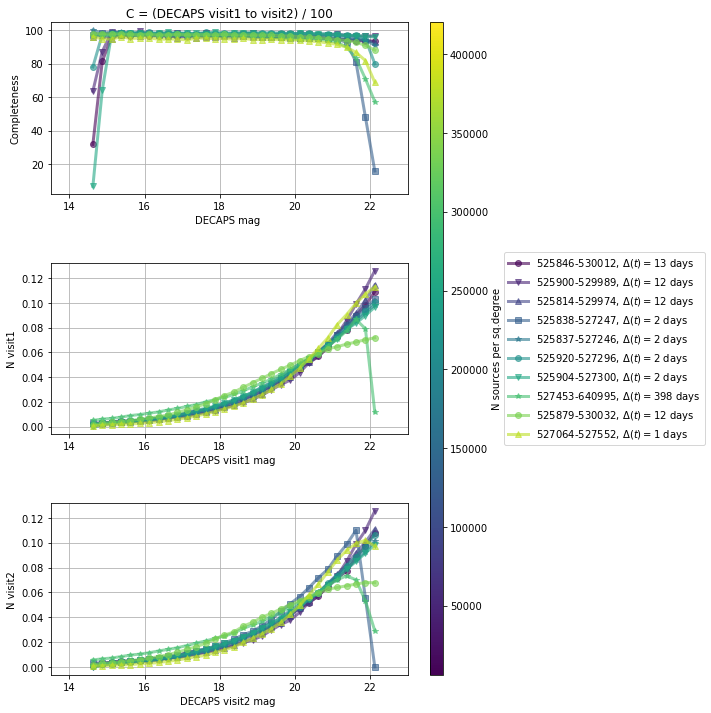
\includegraphics[width=0.75\columnwidth]{figs/completeness_3_decaps.png}
%\vskip -0.15in
\caption{The same quantities as on Fig.~\ref{fig:completeness}, but corresponding to two different visits at the same location, to test the repeatability of DECAPS detections. The two visits (visit1, visit2) were chosen in the same filter and at the same location, and as in tests for completeness, we match source-by-source and consider the number of sources per magnitude bin in visit1 that do have a matching source in visit2. }
\label{fig:completeness_decaps}
\end{centering}
\end{figure} 


% #############################################################
% ###################### PHOTOMETRY  ##########################
% #############################################################


\subsection{Photometry}
\label{sec:photometry}

We consider here photometric accuracy. Since both DECAPS and LSST processing pipelines start from the same instcal calibrated DECam images, they ought arrive at similar measurement of flux, and in turn, instrumental magnitudes.  

An offset and a spread in magnitude difference is due to details of each image processing pipeline.

We compare the photometric repeatability within each pipeline, as well as the existence of offset and spread between two different pipeines. We test pipeline repeatability by investigating two visits at the same locations,  taken in same filters, with equal exposure times.  Assuming that the majority of objects are non-variable in nature, we find the statistical epoch-to-epoch variance. 

\begin{figure}
\begin{centering}
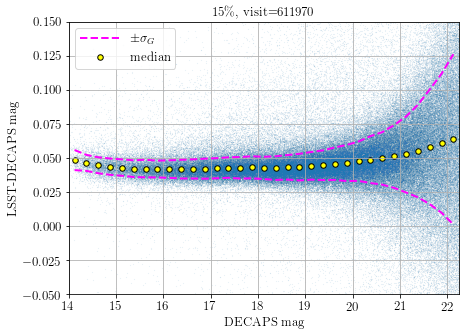
\includegraphics[width=0.6\columnwidth]{figs/15_decaps_lsst_dmag_density_15.png}
%\vskip -0.15in
\caption{Difference in magnitudes between the DECAPS and LSST magnitudes for sources matched within 0.5 \arcsec for a region in top 15\% density (611970) . The magenta dashed line traces the $\pm \sigma_{G}(\Delta m)$ level, and yellow circles the median.  $\sigma_{G} = 0.7413 * (q75 - q25)$, where $q75$ and $q25$ are 75th and 25th percentiles, is an interquartile-based measure of standard deviation, that is insensitive to the outliers. For this stellar density, the offset between LSST and DECAPS is on the level of 0.05 mag. The same quantities ($\sigma_{G}$, median($\Delta m$)) plotted for fields of various stellar densities are shown on Fig.~\ref{fig:lsst_decaps_dmag}. The histograms of $\Delta mag$ per magnitude bin are shown on Fig.~\ref{fig:dmag_hist}.}
\label{fig:dmag_scatter}
\end{centering}
\end{figure} 


\begin{figure}
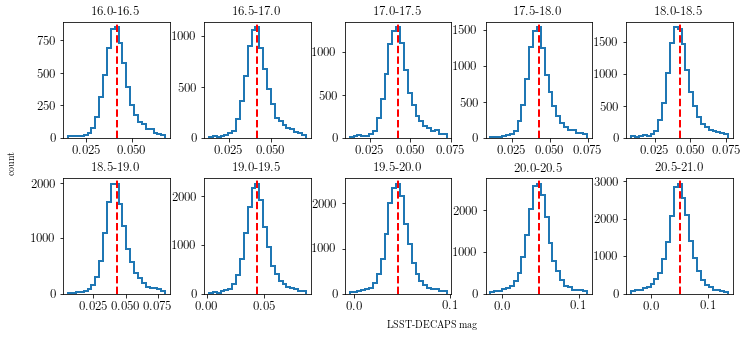
\includegraphics[width=1.0\columnwidth]{figs/16_rms_decaps_lsst_611970hist_panel.png}
%\vskip -0.15in
\caption{Cross-section of Fig.~\ref{fig:dmag_scatter}, showing the histogram of $\Delta mag$ per DECAPS magnitude bin. The vertical red line corresponds to the median value of $\Delta mag$ in that bin, and each histogram is limited between $\pm 4 \, \sigma_{G}$. }
\label{fig:dmag_hist}
\end{figure} 


\begin{figure}
\begin{centering}
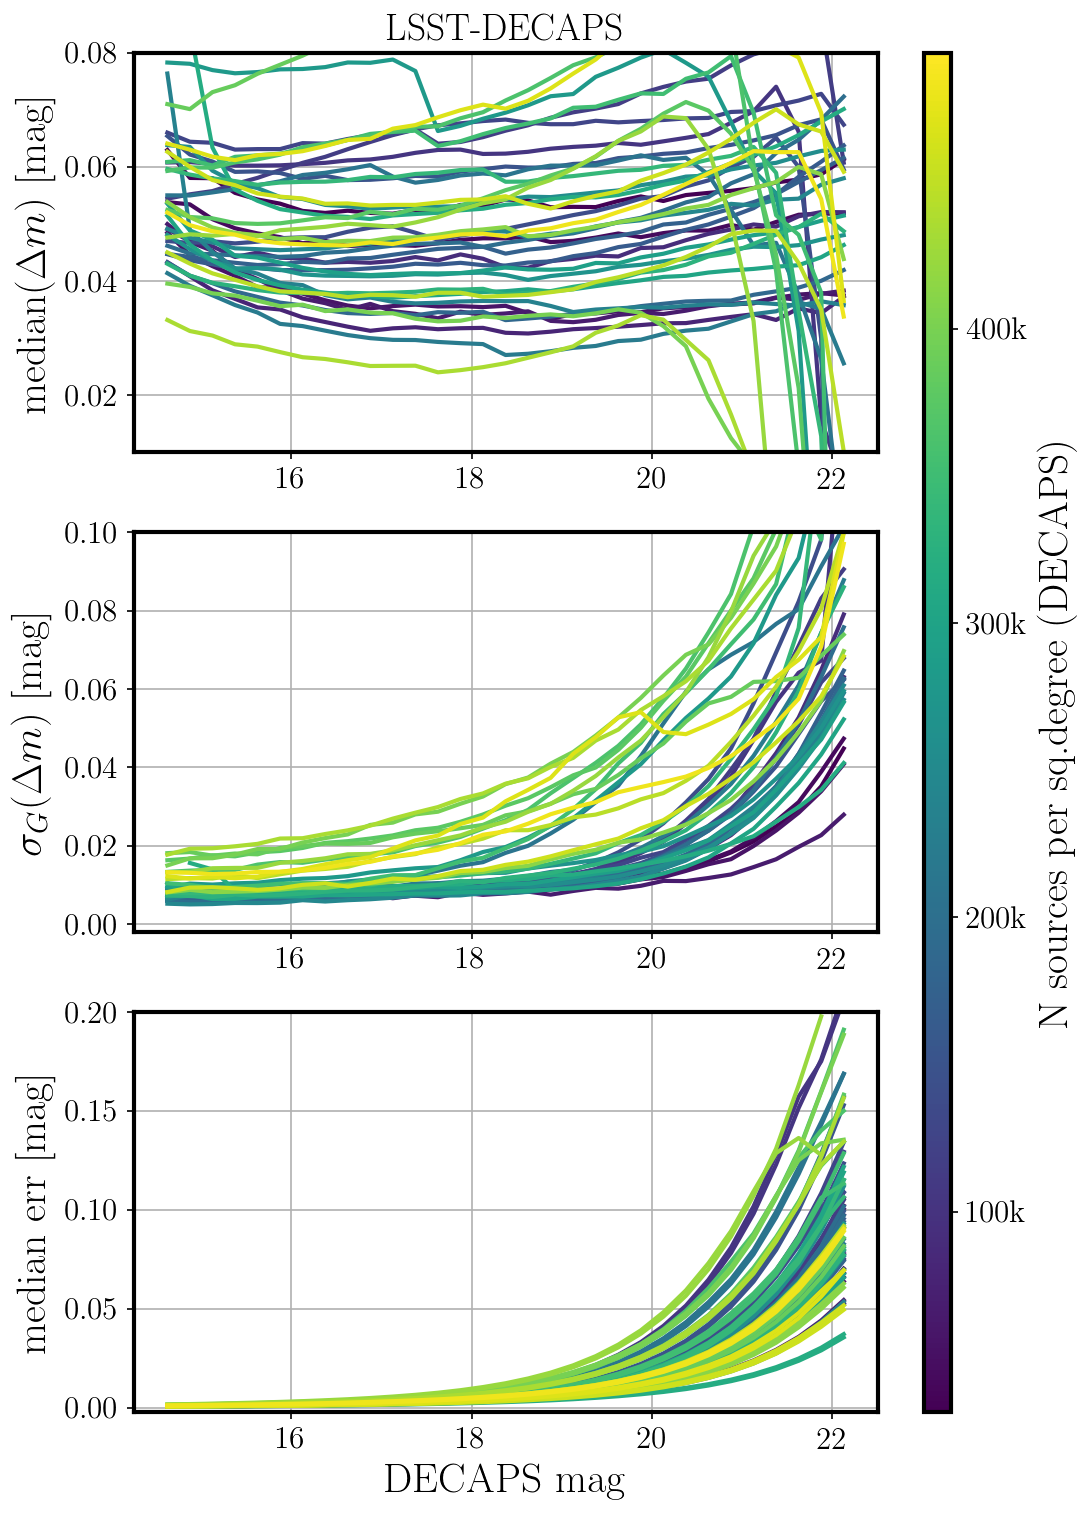
\includegraphics[width=0.7\columnwidth]{figs/decaps_lsst_rms_plot.png}
%\vskip -0.15in
\caption{The measurement of photometric offset between DECAPS and LSST pipelines. For each visit we cross-matched source catalogs corresponding to LSST and DECAPS processing; $\Delta m$ is the difference in magnitude reported between DECAPS and LSST for the same source. For each visit we bin sources according to their DECAPS magnitude. On three panels we plot the binned statistics : median($\Delta m$),  $\sigma_{G}(\Delta m)$, and median photometric uncertainty.}
\label{fig:lsst_decaps_dmag}
\end{centering}
\end{figure} 



Using the DECAPS image database for several visits we found a second visit at exactly the same location, filter and exposure time, but different epoch (see Table ~\ref{tab:epoch12_selection}).  This allowed to test the epoch-epoch photometric repeatability of DECAPS-LSST. We illustrate the  magnitude differences on Figs.~\ref{fig:decaps_decaps_dmag} and \ref{fig:lsst_lsst_dmag}, and the summary of the spread of photometric difference as a function of magnitude on Figs.~\ref{fig:epoch_lsst_multiplot} and ~\ref{fig:epoch_decaps_multiplot}. 


\begin{table}
\centering
\caption{Pairs of visits at two different epochs, arranged by the mean LSST-DECAPS source density (last column). The RA and DEC are in degrees, and mean source density $\langle N_{1,2} \rangle$ in sources per sq. deg.}
\label{tab:epoch12_selection}
\begin{tabular}{ccccccccccc}
\hline
visit1 & ra1 & dec1 & visit2 & ra2 & dec2 & $\langle N_{1,2} \rangle$ \\
\hline
525846 & 133.55 & -44.27 & 530012 & 133.55 & -44.27 & 39733 \\
525900 & 140.62 & -48.15 & 529989 & 140.62 & -48.15 & 44577 \\
525814 & 126.43 & -43.07 & 529974 & 126.42 & -43.07 & 66455 \\
525838 & 132.59 & -50.3 & 527247 & 132.59 & -50.31 & 94766 \\
611969 & 115.53 & -24.08 & 612757 & 115.79 & -24.11 & 106851 \\
525837 & 131.56 & -48.6 & 527246 & 131.56 & -48.6 & 110734 \\
525920 & 143.23 & -51.45 & 527296 & 143.23 & -51.45 & 119371 \\
525904 & 140.55 & -51.25 & 527300 & 140.55 & -51.25 & 138384 \\
641497 & 166.47 & -53.71 & 644035 & 166.73 & -53.8 & 167267 \\
567283 & 247.04 & -47.27 & 645255 & 247.03 & -47.27 & 185894 \\
644082 & 190.31 & -61.09 & 527555 & 190.32 & -61.09 & 186731 \\
527453 & 173.92 & -62.16 & 640995 & 173.91 & -62.16 & 195763 \\
525879 & 137.64 & -54.08 & 530032 & 137.64 & -54.09 & 197058 \\
567795 & 252.15 & -47.43 & 644205 & 251.81 & -47.41 & 211186 \\
527064 & 189.89 & -59.43 & 527552 & 189.88 & -59.43 & 224731 \\
526028 & 168.47 & -56.53 & 641500 & 168.47 & -56.52 & 281929 \\
641548 & 176.18 & -66.43 & 644011 & 176.46 & -66.52 & 336729 \\
644144 & 243.08 & -53.37 & 566793 & 243.08 & -53.37 & 339183 \\
644074 & 188.49 & -67.28 & 644070 & 188.18 & -67.23 & 419000 \\
\hline
\end{tabular}
\end{table}


\begin{figure}
\begin{centering}
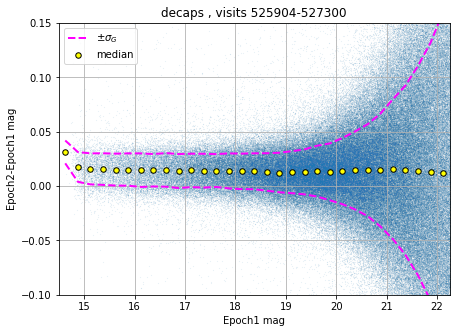
\includegraphics[width=0.7\columnwidth]{figs/18_decaps-decaps525904-527300_dmag.png}
%\vskip -0.15in
\caption{Similarly to Fig.~\ref{fig:dmag_scatter}, scatter plot of the magnitude difference between the two  visits ( 525904, 527300) to the same sky region, separated by 2.95 days, processed by DECAPS. The magnitude difference is shown for all sources cross-matched between  the two epochs, with a match within 0.5\arcsec - there is no selection on magnitude difference, but 0.5 mag (used for completeness) is well beyond the bounds of the plot, and would only remove the outliers to which neither median nor $\sigma_{G}$ are sensitive.  We overplot the $\pm \sigma_{G}$ envelope, and the median of each 0.25 mag bin. }
\label{fig:decaps_decaps_dmag}
\end{centering}
\end{figure} 


\begin{figure}
\begin{centering}
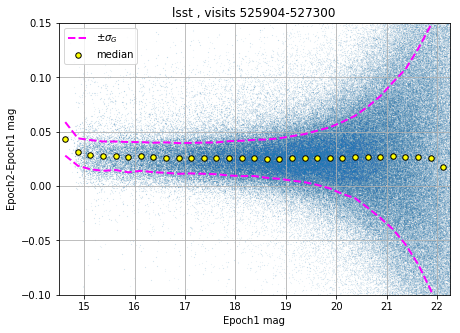
\includegraphics[width=0.7\columnwidth]{figs/19_lsst-lsst525904-527300_dmag.png}
%\vskip -0.15in
\caption{The same as Fig.~\ref{fig:decaps_decaps_dmag}, but for LSST processing of  two visits to the same region, at two different epochs. }
\label{fig:lsst_lsst_dmag}
\end{centering}
\end{figure} 


\begin{figure}
\begin{centering}
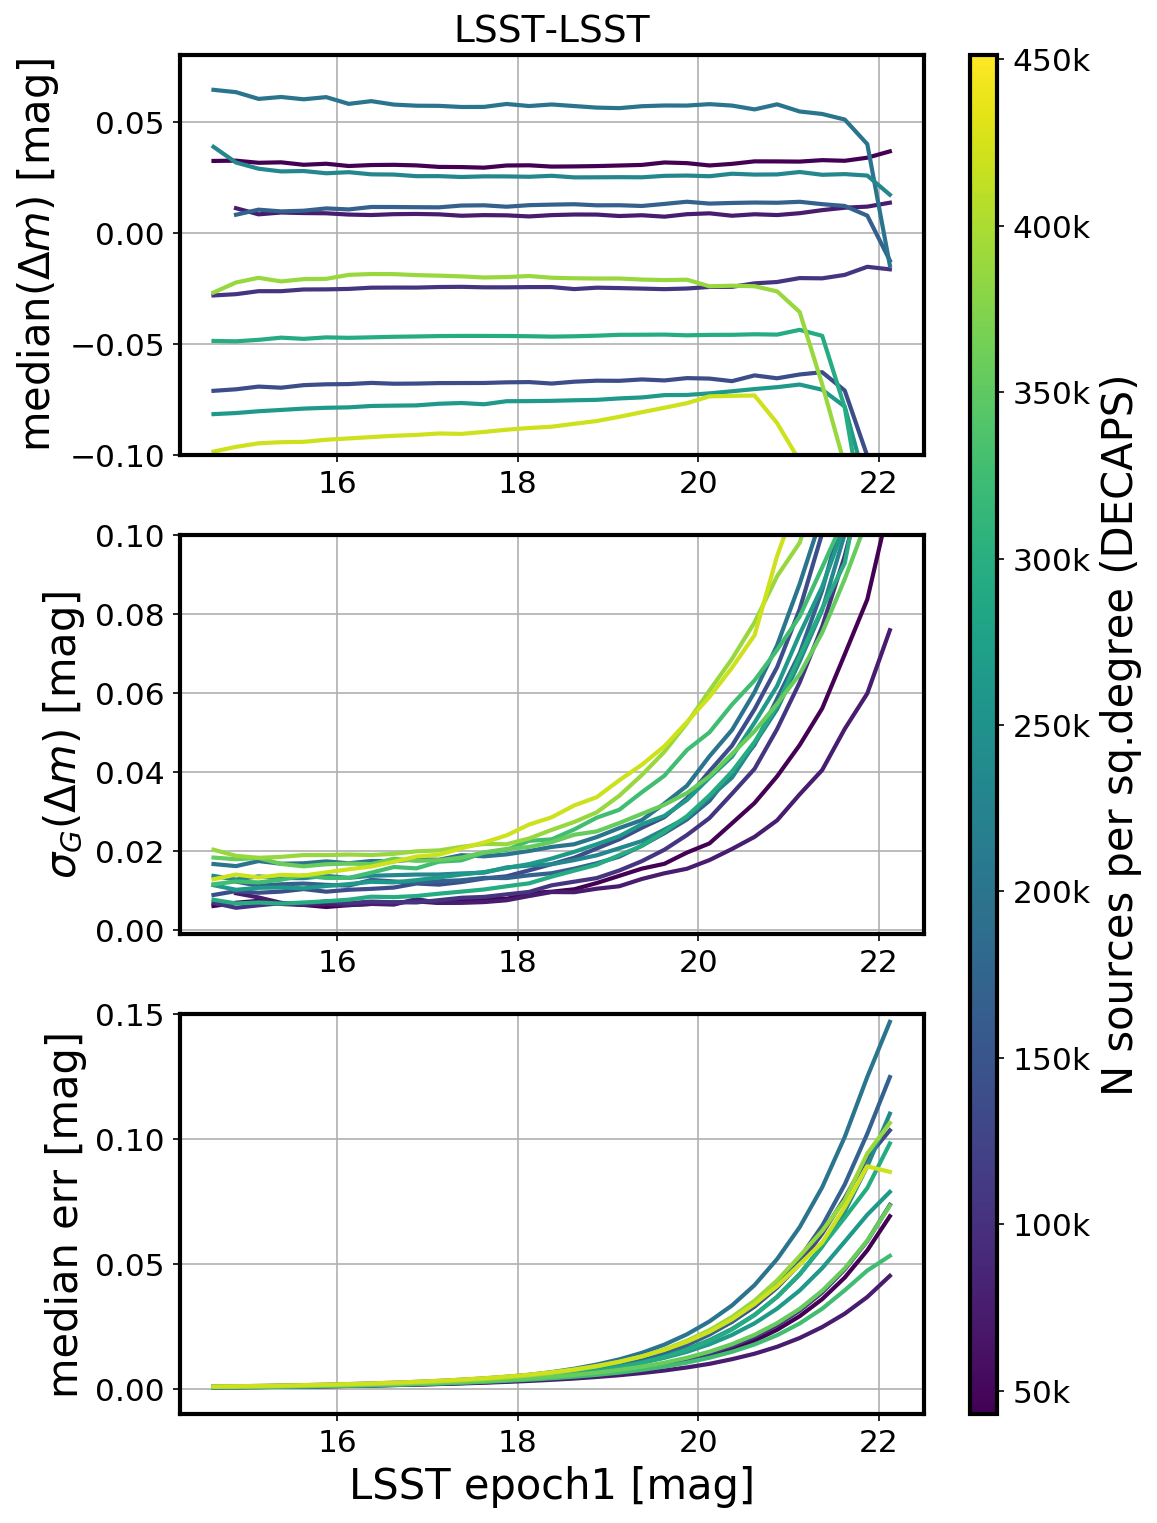
\includegraphics[width=0.8\columnwidth]{figs/lsst-lsst_rms_plot.png}
%\vskip -0.15in
\caption{The internal repeatability test of the LSST pipeline. We cross-match the source catalogs for each visit. These two brightness measurements for the same source are akin to a two-epoch light curve. Since inherently variable sources constitute a small fraction of all stellar objects, and the majority of stars are not variable, the difference in the measured magnitudes would correspond to the empirical measure of noise.  All sources cross-matched within 0.5\arcsec are binned according to their brightness. On the panels we plot, from top to bottom: median photometric offset, the robust interquartile-based measure of standard deviation $\sigma_{G}$, and the median reported measurement uncertainty.}
\label{fig:epoch_lsst_multiplot}
\end{centering}
\end{figure} 


\begin{figure}
\begin{centering}
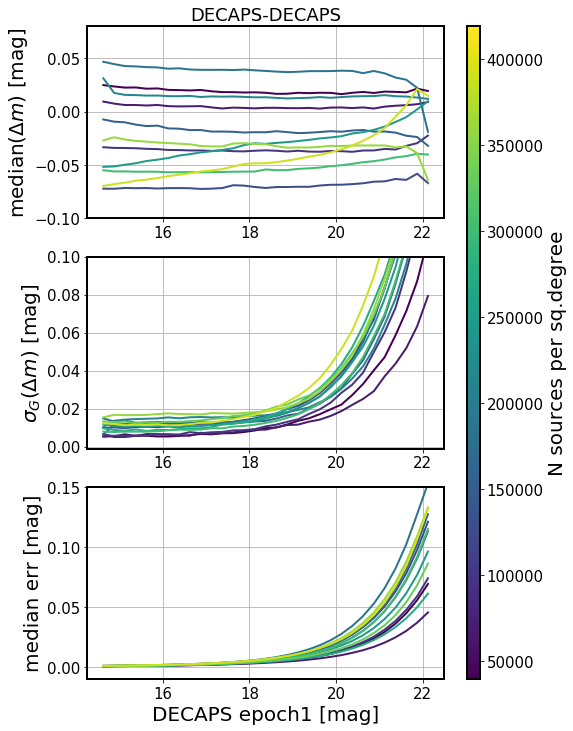
\includegraphics[width=0.8\columnwidth]{figs/decaps-decaps_rms_plot.png}
%\vskip -0.15in
\caption{The internal repeatability test of DECAPS pipeline - for description, see Fig.~\ref{fig:epoch_lsst_multiplot}.}
\label{fig:epoch_decaps_multiplot}
\end{centering}
\end{figure} 

We summarize the information about the photometric repeatability (epoch-to-epoch within a given pipeline), and offset (pipeline-to-pipeline of the same epoch), by combining information from  Figs.~\ref{fig:lsst_decaps_dmag},~\ref{fig:epoch_lsst_multiplot}, ~\ref{fig:epoch_decaps_multiplot}. In particular, we characterize the photometric accuracy by a systematic offset between the emipirical measure of noise and the pipeline-reported photometric uncertainty (Figs.~\ref{fig:spread_1},~\ref{fig:spread_2},~\ref{fig:spread_summary}).



\begin{figure}
\begin{centering}
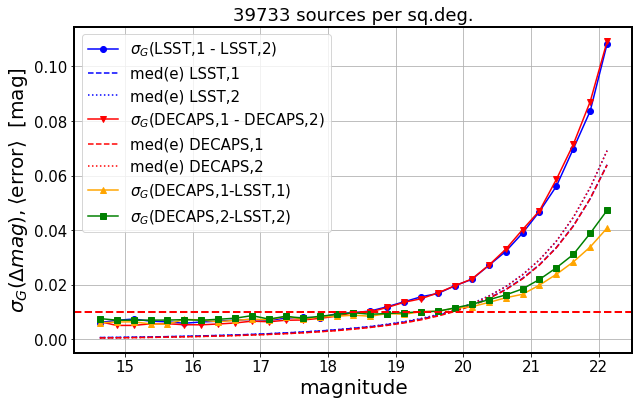
\includegraphics[width=0.8\columnwidth]{figs/photometric_spread_1_525846-530012.png}
%\vskip -0.15in
\caption{Comparison of spread of scatter between two pipelines vs.  the empirical measurement of noise from repeatability for a pair of visits at the same location : 525846 and 530012, here called epoch1 and epoch2. All solid lines are $\sigma_{G}(a,b)$ - the interquartile-based measure of spread of magnitude difference between measurements $a$ and $b$ of the same source. From the top,  $\sigma_{G}(LSST,1 - LSST,2)$, and $\sigma_{G}(DECAPS,1 - DECAPS,2)$, correspond to the empirical measure of noise.  The blue line  $\sigma_{G}(LSST,1 - LSST,2)$ is the same quantity as that plotted on the middle panel of Fig.~\ref{fig:epoch_lsst_multiplot}, while the red line  $\sigma_{G}(DECAPS,1 - DECAPS,2)$ is the same as that of Fig.~\ref{fig:epoch_decaps_multiplot}. Then the dotted and dashed lines in the middle show the median error for epoch 1 or epoch 2, as reported by LSST or DECAPS pipelines. They represent the expected uncertainty in repeated measurement.  Since they are identical, the red and blue dotted or dashed lines overlap.  Finally, the green and orange solid curves correspond to the scatter between the two pipelines , calculated either for epoch1 ($\sigma_{G}(DECAPS,1 - LSST,1)$), or epoch2 ($\sigma_{G}(DECAPS,2- LSST,2)$). Fig.~\ref{fig:spread_2} shows the second step in the analysis. }
\label{fig:spread_1}
\end{centering}
\end{figure} 


\begin{figure}
\begin{centering}
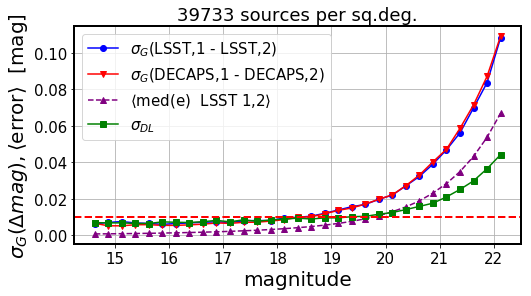
\includegraphics[width=0.8\columnwidth]{figs/photometric_spread_2_525846-530012.png}
%\vskip -0.15in
\caption{Second step in the analysis of  photometric spread, following Fig.~\ref{fig:spread_1}. The blue and red lines of repeatability are unchanged.  Since LSST and DECAPS errors are almost identical, we choose to represent the minimum statistical offset by the mean LSST error between the two visits , added in quadrature . If $e_{1L}$ and $e_{2L}$ are LSST-reported error measurements for a given source for the two epochs,  the quadrature-mean is  $e_{12} = \sqrt{e_{1L}^{2} + e_{2L}^{2}} / \sqrt{2}$, and the purple dashed line is the median of $e_{12}$ per magnitude bin.    We also add in quadrature the spread between the two pipelines, represented  on Fig.~\ref{fig:spread_1} by orange $\sigma_{DL,1}$ for epoch1, and green $\sigma_{DL,2}$ for epoch2 : $\sigma_{DL} = \sqrt{\sigma_{DL,1}^{2} + \sigma_{DL,2}^{2}} / \sqrt{2}$.  Note that since the top blue (or red) lines $\sigma_{G}(LSST,1 - LSST,2)$, $\sigma_{G}(DECAPS,1 - DECAPS,2)$   ($\sigma_{DD}$, $\sigma_{LL}$ for short) consists of noise $\sigma_{E} $ and the systematic offset $\sigma_{S}$ : $\sigma_{LL}^{2} = \sigma_{S}^{2} + \sigma_{E}^{2}$. Thus we calculate the systematic offset for LSST as  $\sigma_{S} = \sqrt{\sigma_{LL}^2  - \sigma_{E}^{2}}$, which is the difference between  blue solid and purple dashed lines. 
}
\label{fig:spread_2}
\end{centering}
\end{figure} 



\begin{figure}
\begin{centering}
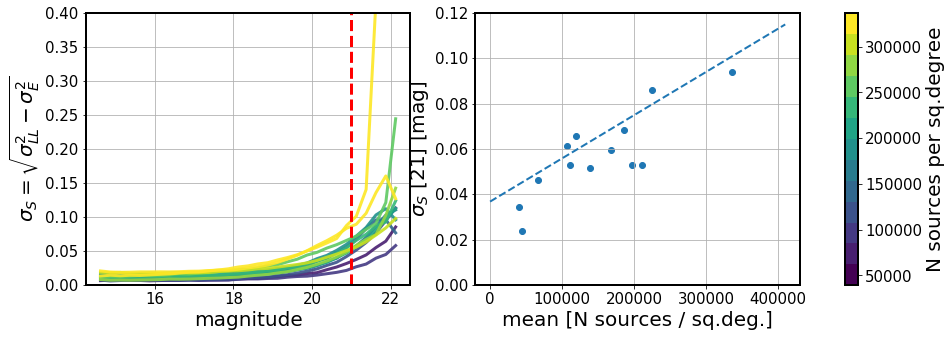
\includegraphics[width=0.95\columnwidth]{figs/photometric_offset_combined.png}
%\vskip -0.15in
\caption{The left panel shows the measure of systematic offset between mean photometric error, and the photometric repeatability for the LSST pipeline as a function of magnitude (see Figs.~\ref{fig:spread_1},~\ref{fig:spread_2}. Colors correspond to mean stellar density. Right panel shows $\sigma_{S}$ at 21st magnitude  as a function of stellar density.}
\label{fig:spread_summary}
\end{centering}
\end{figure} 

% #############################################################
% ###################### ASTROMETRY  ##########################
% #############################################################

\section{Astrometry}
\label{sec:astrometry}
Astrometry pertains to the measurement of the position of sources in the absolute World Coordinate System (WCS). Accurate and precise astrometry enables catalog cross-matching, and over long-term - measurement of proper motion of stellar sources. 

We consider two properties of successful astrometry. First, the internal consistency of a pipeline by measuring the repeatability of astrometric measurement between different epochs.  Second - accuracy, and any biases between the LSST-DECAPS pipelines. 

Part of the astrometric offset between the two pipelines is because  DECAPS employed 2MASS-GAIA data (Fig.12 in ~\cite{schlafly2017}), whereas LSST used GAIA-TGAS data for astrometric calibration. 

In all analysis the RA difference is corrected for the cosine of RA : $\Delta \alpha_{corr} = \delta \alpha \cos{(\delta)}$ % ### add comment why ?  

To test the repeatability we use pairs of observations at the same location, as in Sec.~\ref{sec:photometry}. Fig.~\ref{fig:ra_dec_lsst_lsst} shows an example of the LSST-LSST comparison, with Fig.~\ref{fig:ra_dec_mag} showing the magnitude dependence. Fig.~\ref{fig:ra_dec_decaps_decaps} depicts the offset in $RA$, $DEC$, for DECAPS-DECAPS comparison. 


To test possible offset between LSST and DECAPS astrometric solutions, on Fig.~\ref{fig:ra_dec_lsst_decaps} we find the offset in measured $RA$, $DEC$ for sources cross-matched in catalogs from the two pipelines. 

\begin{figure}
\begin{centering}
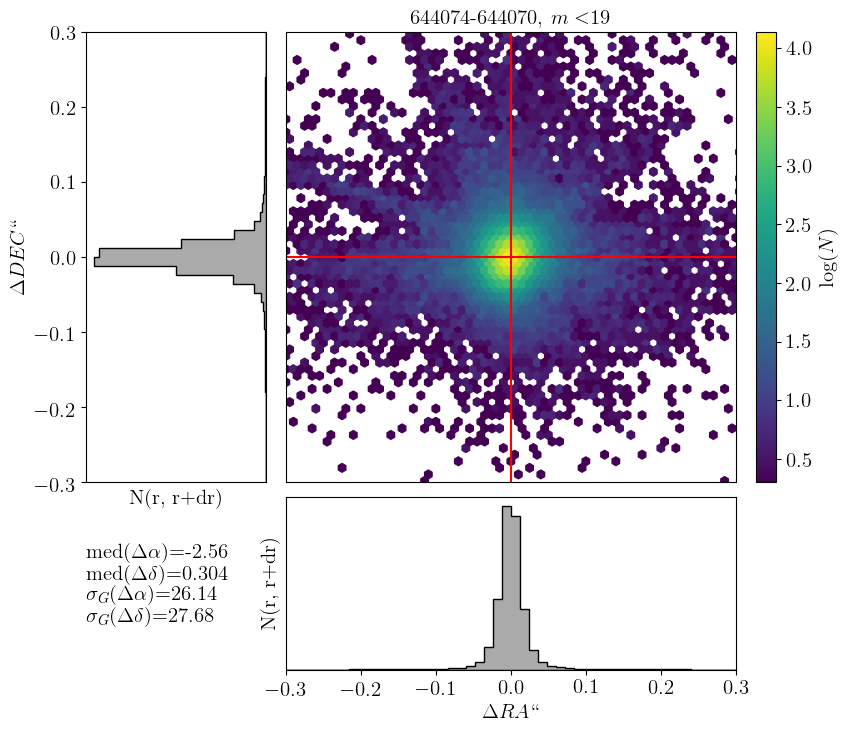
\includegraphics[width=0.8\columnwidth]{figs/lsst644074-644070_RA_DEC_offset_lims.png}
%\vskip -0.15in
\caption{The difference of LSST processing for  RA,DEC for visits 644074,644070: a pair of visits at the same location, separated by less than a day. The mean number of sources is 419000 sources per sq.deg., which corresponds to top 1\% of the sky.  We select sources brighter than 19 magnitude.  For all other pairs the  offsets are all centered on zero with similar spread - see Table~\ref{tab:radec_lsst_lsst}}
\label{fig:ra_dec_lsst_lsst}
\end{centering}
\end{figure} 


\begin{figure}
\begin{centering}
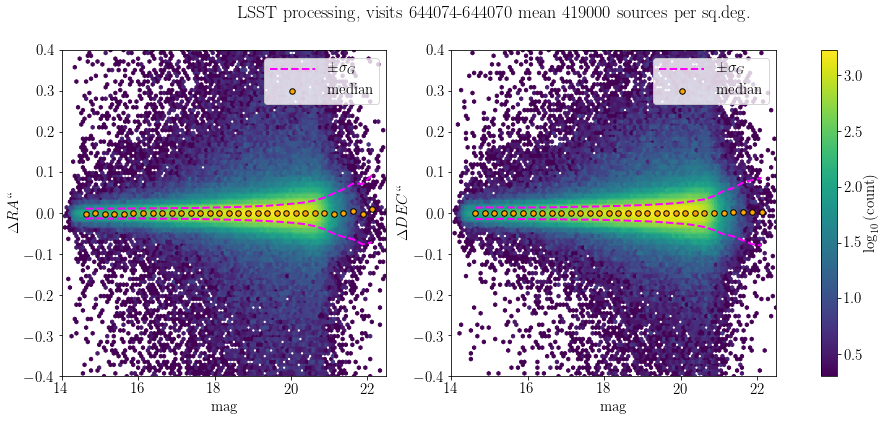
\includegraphics[width=1.0\columnwidth]{figs/644074-644070_dra_ddec_mag.png}
%\vskip -0.15in
\caption{The difference in RA,DEC for the same visits as on Fig.~\ref{fig:ra_dec_lsst_lsst}, shown as a function of magnitude.}
\label{fig:ra_dec_mag}
\end{centering}
\end{figure} 



\begin{table}
\centering
\caption{The difference in RA,DEC for various visits, between LSST processing of fields at the same location, but observed at different times ( see Table ~\ref{tab:epoch12_selection} for summary). The median and spread of astrometric offset are in  miliarcseconds. The final column shows the LSST source count averaged between the two visits in counts per square degree.}
\label{tab:radec_lsst_lsst}
\begin{tabular}{ccccccc}
visit1 & visit2 & $\mathrm{med}(\Delta\alpha)$ & $\mathrm{med}(\Delta\delta)$ & $\sigma_{G}(\Delta\alpha)$ & $\sigma_{G}(\Delta\delta)$ & $\langle N \rangle$ \\
525846 & 530012 & 1.83 & 0.18 & 9.43 & 8.85 & 39733 \\
525900 & 529989 & -3.12 & 0.36 & 10.87 & 11.58 & 44577 \\
525814 & 529974 & -0.29 & 1.15 & 10.65 & 10.46 & 66455 \\
525838 & 527247 & 2.52 & -2.23 & 9.96 & 12.21 & 94766 \\
525837 & 527246 & 1.58 & -1.24 & 9.07 & 11.51 & 110734 \\
525920 & 527296 & 0.88 & -3.2 & 10.36 & 9.85 & 119371 \\
525904 & 527300 & 0.43 & -1.55 & 8.29 & 10.0 & 138384 \\
641497 & 644035 & 2.26 & -1.42 & 19.8 & 22.68 & 167267 \\
567283 & 645255 & -5.58 & 1.05 & 33.77 & 19.75 & 185894 \\
644082 & 527555 & -4.16 & -5.05 & 29.92 & 26.1 & 186731 \\
527453 & 640995 & -0.33 & 1.7 & 12.95 & 12.25 & 195763 \\
525879 & 530032 & 0.8 & -0.46 & 10.56 & 13.41 & 197058 \\
527064 & 527552 & -0.13 & -2.19 & 16.93 & 15.74 & 224731 \\
526028 & 641500 & -1.2 & 0.42 & 11.52 & 11.12 & 281929 \\
641548 & 644011 & 1.2 & -2.43 & 26.08 & 30.7 & 336729 \\
644144 & 566793 & 1.05 & -0.25 & 27.86 & 19.69 & 339183 \\
644074 & 644070 & -2.56 & 0.3 & 26.14 & 27.69 & 419000 \\
\end{tabular}
\end{table}



\begin{figure}
\begin{centering}
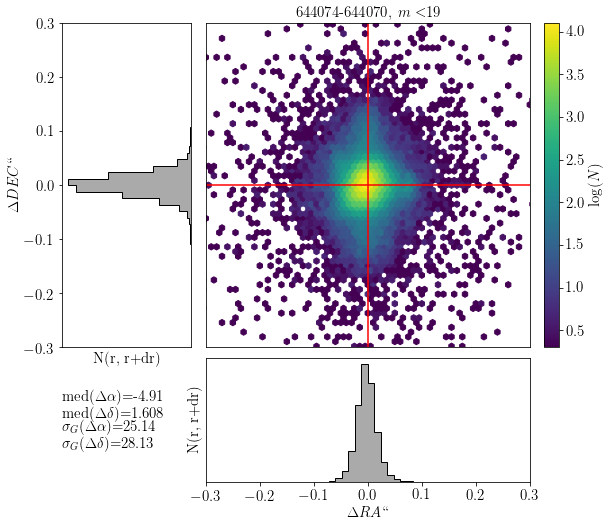
\includegraphics[width=0.8\columnwidth]{figs/decaps644074-644070_RA_DEC_offset_lims.png}
%\vskip -0.15in
\caption{The difference in RA,DEC for  the same visits as in Fig.~\ref{fig:ra_dec_lsst_lsst}, but comparing DECAPS single-epoch catalogs. The spread of  $\Delta \alpha$, $\Delta \delta$ is wider than for equivalent visit pairs processed by the LSST Science Pipelines - see Table~\ref{tab:radec_decaps_decaps}}
\label{fig:ra_dec_decaps_decaps}
\end{centering}
\end{figure} 



\begin{table}
\centering
\caption{The difference in RA,DEC for various visits, between DECAPS processing of fields at the same location, but observed at different times ( see Table ~\ref{tab:epoch12_selection} for summary). All  measured quantities are in miliarcseconds. See Table ~\ref{tab:radec_lsst_lsst} for the equivalent visits processed by LSST. }
\label{tab:radec_decaps_decaps}
\begin{tabular}{ccccccc}
visit1 & visit2 & $\mathrm{med}(\Delta\alpha)$ & $\mathrm{med}(\Delta\delta)$ & $\sigma_{G}(\Delta\alpha)$ & $\sigma_{G}(\Delta\delta)$ & $\langle N \rangle$ \\
525846 & 530012 & 5.92 & -1.18 & 14.69 & 14.49 & 39733 \\
525900 & 529989 & -5.34 & -4.18 & 21.18 & 20.76 & 44577 \\
525814 & 529974 & 6.55 & 0.19 & 20.58 & 17.76 & 66455 \\
525838 & 527247 & -6.5 & -0.72 & 17.62 & 16.45 & 94766 \\
525837 & 527246 & -3.55 & -2.86 & 18.5 & 17.57 & 110734 \\
525920 & 527296 & -4.97 & -3.26 & 19.72 & 16.88 & 119371 \\
525904 & 527300 & -5.05 & -4.13 & 14.4 & 16.26 & 138384 \\
641497 & 644035 & 8.91 & 12.57 & 34.18 & 31.02 & 167267 \\
567283 & 645255 & -53.12 & -49.23 & 39.71 & 24.55 & 185894 \\
644082 & 527555 & 139.33 & -15.63 & 40.71 & 36.27 & 186731 \\
527453 & 640995 & -126.51 & 28.81 & 24.75 & 18.27 & 195763 \\
525879 & 530032 & -0.43 & -5.17 & 22.88 & 23.66 & 197058 \\
527064 & 527552 & 5.11 & -3.74 & 20.95 & 25.13 & 224731 \\
526028 & 641500 & -134.26 & 28.5 & 26.81 & 19.56 & 281929 \\
641548 & 644011 & -1.69 & -5.63 & 32.3 & 36.95 & 336729 \\
644144 & 566793 & 94.95 & 68.82 & 32.42 & 23.74 & 339183 \\
644074 & 644070 & -4.92 & 1.61 & 25.15 & 28.14 & 419000 \\
\end{tabular}
\end{table}






\begin{figure}
\begin{centering}
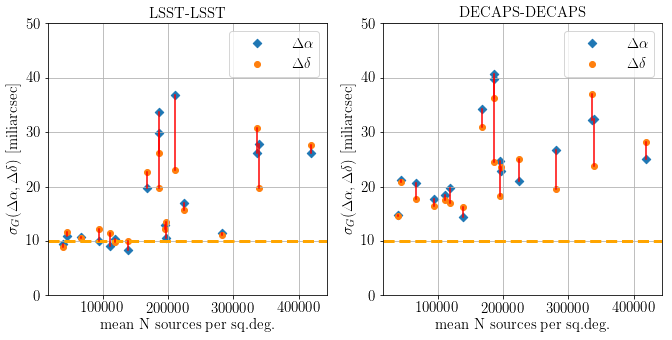
\includegraphics[width=0.8\columnwidth]{figs/Astrometry_LSST-LSST_DECAPS-DECAPS.png}
%\vskip -0.15in
\caption{Summary of LSST and DECAPS repeatability of astrometry, as in Tables ~\ref{tab:radec_lsst_lsst} and ~\ref{tab:radec_decaps_decaps}.}
\label{fig:lsst_decaps_side}
\end{centering}
\end{figure} 


\begin{figure}
\begin{centering}
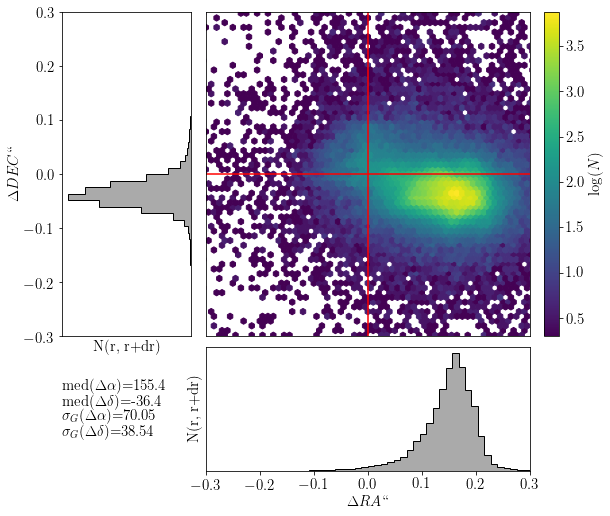
\includegraphics[width=0.8\columnwidth]{figs/22_525904_RA_DEC_offset.png}
%\vskip -0.15in
\caption{The difference in RA,DEC for visit 525904 , between LSST and DECAPS processing (402270 detected sources in  the clean LSST catalog ). We tested that for other vists and in all cases the offset position and magnitude remains the same - see Table~\ref{tab:radec_lsst_decaps}}
\label{fig:ra_dec_lsst_decaps}
\end{centering}
\end{figure} 


\begin{table}
\centering
\caption{The difference in RA,DEC for the same visit analyzed by LSST and DECAPS.  Each row corresponds to a separate visit, which correspond to different stellar density.  All  measured quantities are in miliarcseconds. }
\label{tab:radec_lsst_decaps}
\begin{tabular}{ccccc}
visit & $\mathrm{median}(\Delta\alpha)$ & $\mathrm{median}(\Delta\delta)$ & $\sigma_{G}(\Delta\alpha)$ & $\sigma_{G}(\Delta\delta)$ \\
\hline
525904 & 155.49 & -36.46 & 70.06 & 38.55 \\
525920 & 130.45 & -27.53 & 72.83 & 43.88 \\
525846 & 105.62 & -51.71 & 42.49 & 30.04 \\
525879 & 131.93 & -42.62 & 138.58 & 75.68 \\
525837 & 96.01 & -47.93 & 65.17 & 36.6 \\
525838 & 124.9 & -68.92 & 59.56 & 33.99 \\
525814 & 39.99 & -29.87 & 47.26 & 29.72 \\
525900 & 127.61 & -32.38 & 54.81 & 33.67 \\
527300 & 146.26 & -38.73 & 56.49 & 25.48 \\
527296 & 120.47 & -26.98 & 41.65 & 27.14 \\
530012 & 111.21 & -51.38 & 35.01 & 28.34 \\
530032 & 126.69 & -47.85 & 115.02 & 65.23 \\
527246 & 88.38 & -49.06 & 45.87 & 30.6 \\
527247 & 110.44 & -66.18 & 43.15 & 29.71 \\
529974 & 49.13 & -30.91 & 48.55 & 28.95 \\
529989 & 126.51 & -33.77 & 52.12 & 28.33 \\
\end{tabular}
\end{table}




\section{Conclusions}
\label{sec:conclusions}

% ### need to add things here ... 

\subsection{LSST Processing of StarFast Simulated Sky}
An independent way to further test the performance of the LSST Science Pipelines is to use the simulated sky images, where the true position and  brightness of each source is known. This would put the measure of source detection completeness, photometric and astrometric precision on an absolute scale. We already tested a StarFast image simulator\footnote{\url{https://dmtn-012.lsst.io}}, and confirmed that it can successfully simulate a region of the sky seeded with known stellar population.  


\subsection{Other LSST-DECAPS tests: w-color }
An independent test of the quality of photometry would be to consider the width of the stellar locus ('w-color') on the g-r vs r-i color-color plot.  This could be used to test internal consistency of LSST and DECAPS photometry. 


%%%%%%%%%%%%%%%%%%%%%%%%%%%%%%%%%%%%%%%%%%%%%%%%%%
%%%%%%%%%%%%%%%%%%%% REFERENCES %%%%%%%%%%%%%%%%%%
%%%%%%%%%%%%%%%%%%%%%%%%%%%%%%%%%%%%%%%%%%%%%%%%%%

\bibliographystyle{apj}
\bibliography{references}
\end{document}